\documentclass[aspectratio=169,10pt]{beamer}

\usepackage[T2A]{fontenc}
\usepackage[utf8]{inputenc}
\usepackage[russian]{babel}
\usepackage{amsmath,amssymb,amsfonts}
\usepackage{booktabs}
\usepackage{array}
\usepackage{graphicx}

\usetheme{Madrid}
\usecolortheme{default}
\setbeamertemplate{navigation symbols}{}
\setbeamertemplate{caption}[numbered]
\graphicspath{{images_presentation/}}

\definecolor{mainblue}{RGB}{25,70,145}
\setbeamercolor{structure}{fg=mainblue}
\setbeamercolor{frametitle}{fg=white,bg=mainblue}

\newcommand{\Reynolds}{\operatorname{Re}}
\newcommand{\Laplace}{\Delta}
\newcommand{\norm}[1]{\left\lVert #1 \right\rVert}
\newcommand{\inner}[2]{\left\langle #1,#2 \right\rangle}
\newcommand{\J}{J}

\title[Стабилизация в переменных \(\psi,\omega\)]{Задача стабилизации для задачи магнитной гидродинамики\\в переменных \((\psi,\omega)\)}
\author{Выполнил студент 431 группы\\Сенцов Александр Артёмович\\[0.6em]
Научный руководитель\\Корнев Андрей Алексеевич}
\institute{Механико-математический факультет МГУ}
\date{2026}

\begin{document}

\begin{frame}
    \titlepage
\end{frame}

\begin{frame}{Постановка задачи: уравнения Навье--Стокса}
    Рассматривается двумерное течение несжимаемой вязкой жидкости:
    \[
        \frac{\partial \mathbf u}{\partial t}
        +
        (\mathbf u\cdot\nabla)\mathbf u
        =
        -\nabla p
        +
        \nu\Laplace \mathbf u
        +
        \mathbf f,
        \qquad
        \nabla\cdot\mathbf u=0.
    \]
    Здесь
    \[
        \mathbf u=(u,v),\qquad
        p=p(x,y,t),\qquad
        \nu=\frac{1}{\Reynolds}.
    \]
    Давление исключается переходом к завихренности.
    В двумерном случае используется скалярная завихренность
    \[
        \omega = v_x-u_y.
    \]
\end{frame}

\begin{frame}{Переход к переменным \((\psi,\omega)\)}
    Скорость выражается через функцию тока:
    \[
        u=\psi_y,\qquad v=-\psi_x,\qquad
        \operatorname{div}\mathbf u=0.
    \]
    Связь функции тока и завихренности:
    \[
        \Laplace\psi+\omega=0.
    \]
    После применения операции ротора к уравнениям Навье--Стокса получается уравнение для завихренности:
    \[
        \omega_t
        =
        \nu\Laplace\omega
        -
        \J(\psi,\omega)
        -
        F_\omega(x,y),
        \qquad
        \J(\psi,\omega)=\psi_x\omega_y-\psi_y\omega_x.
    \]
    Далее численно решается система
    \[
        \begin{cases}
        \Laplace\psi+\omega=0,\\
        \omega_t=\nu\Laplace\omega-\J(\psi,\omega)-F_\omega(x,y).
        \end{cases}
    \]
\end{frame}

\begin{frame}{Общие граничные условия}
    На твёрдой непроницаемой стенке функция тока постоянна:
    \[
        \psi\big|_{\partial\Omega}=\mathrm{const}.
    \]
    Для односвязной замкнутой области константа выбирается нулевой:
    \[
        \psi\big|_{\partial\Omega}=0.
    \]
    Завихренность на стенке не задаётся независимо, а восстанавливается из условия прилипания.
    Для горизонтальной стенки с тангенциальной скоростью \(U\):
    \[
        \omega_{\mathrm{wall}}
        =
        -\frac{2\psi_{\mathrm{near}}}{h^2}
        -
        \frac{2U}{h}.
    \]
    Это формула Тома для связи граничной завихренности с ближайшим внутренним значением \(\psi\).
\end{frame}

\begin{frame}{Откуда возникает якобиан}
    Нелинейность в уравнении завихренности связана с переносом завихренности полем скорости:
    \[
        (\mathbf u\cdot\nabla)\omega
        =
        u\omega_x+v\omega_y.
    \]
    После подстановки
    \[
        u=\psi_y,\qquad v=-\psi_x
    \]
    этот член записывается через якобиан двух сеточных функций:
    \[
        \J(\psi,\omega)
        =
        \psi_x\omega_y-\psi_y\omega_x.
    \]
    В задаче о каверне используется центральная аппроксимация:
    \[
        \J_h^{(c)}=(D_x\psi)(D_y\omega)-(D_y\psi)(D_x\omega).
    \]
    В четырёхвихревой задаче этот же член заменяется на схему Аракавы.
\end{frame}

\begin{frame}{Разностные операторы}
    Равномерная сетка:
    \[
        x_i=ih_x,\qquad y_j=jh_y.
    \]
    Центральные разности:
    \[
        (D_x f)_{ij}=\frac{f_{i+1,j}-f_{i-1,j}}{2h_x},
        \qquad
        (D_y f)_{ij}=\frac{f_{i,j+1}-f_{i,j-1}}{2h_y}.
    \]
    Пятиточечный лапласиан:
    \[
        (\Laplace_h f)_{ij}
        =
        \frac{f_{i+1,j}-2f_{ij}+f_{i-1,j}}{h_x^2}
        +
        \frac{f_{i,j+1}-2f_{ij}+f_{i,j-1}}{h_y^2}.
    \]
\end{frame}

\begin{frame}{Факторизованная схема для \(\psi\)}
    Для связи \(\psi\) и \(\omega\) используется псевдовременной процесс:
    \[
        \psi_t=\Laplace_h\psi+\omega.
    \]
    Неявный шаг заменяется факторизованным:
    \[
        (I-\tau D_{xx})(I-\tau D_{yy})\psi^{n+1}
        =
        \psi^n+\tau\omega^n+\tau^2D_{xx}D_{yy}\psi^n.
    \]
    Множитель факторизации:
    \[
        (I-\tau D_{xx})(I-\tau D_{yy})
        =
        I-\tau\Laplace_h+\tau^2D_{xx}D_{yy}.
    \]
    Член \(\tau^2D_{xx}D_{yy}\psi^n\) компенсирует смешанный член факторизации в стационарном пределе.
\end{frame}

\begin{frame}{Две прогонки для \(\psi\)}
    Вводится промежуточное поле \(\psi^*\).
    Первый одномерный шаг выполняется по \(x\):
    \[
        (I-\tau D_{xx})\psi^{*}
        =
        \psi^n+\tau\omega^n+\tau^2D_{xx}D_{yy}\psi^n.
    \]
    Второй одномерный шаг выполняется по \(y\):
    \[
        (I-\tau D_{yy})\psi^{n+1}=\psi^{*}.
    \]
    На каждом подшаге для фиксированной строки или столбца получается трёхдиагональная система.
\end{frame}

\begin{frame}{Схема для \(\omega\) и метод прогонки}
    Факторизованный шаг для завихренности:
    \[
        (I-\tfrac{\tau}{\Reynolds}D_{xx})
        (I-\tfrac{\tau}{\Reynolds}D_{yy})\omega^{n+1}
        =
        \omega^n-\tau \J_h(\psi^n,\omega^n)-\tau F_\omega
        +
        \frac{\tau^2}{\Reynolds^2}D_{xx}D_{yy}\omega^n.
    \]
    После факторизации решаются наборы трёхдиагональных систем:
    \[
        a_iq_{i-1}+c_iq_i+b_iq_{i+1}=d_i.
    \]
    Прогонка:
    \[
        \alpha_i=-\frac{b_i}{c_i+a_i\alpha_{i-1}},
        \qquad
        \beta_i=\frac{d_i-a_i\beta_{i-1}}{c_i+a_i\alpha_{i-1}},
        \qquad
        q_i=\alpha_iq_{i+1}+\beta_i.
    \]
\end{frame}

\begin{frame}{Две прогонки для \(\omega\)}
    Вводится промежуточное поле \(\omega^*\).
    Первый подшаг:
    \[
        (I-\tfrac{\tau}{\Reynolds}D_{xx})\omega^{*}
        =
        \omega^n-\tau \J_h(\psi^n,\omega^n)-\tau F_\omega
        +
        \frac{\tau^2}{\Reynolds^2}D_{xx}D_{yy}\omega^n.
    \]
    Второй подшаг:
    \[
        (I-\tfrac{\tau}{\Reynolds}D_{yy})\omega^{n+1}=\omega^{*}.
    \]
    Нелинейный перенос и внешняя сила находятся в правой части; диффузионная часть обрабатывается неявно по направлениям.
\end{frame}

\begin{frame}{Схема Аракавы}
    Для четырёхвихревого эксперимента используется симметризованный якобиан:
    \[
        \J_h^A(\psi,\omega)
        =
        \frac{1}{3}
        \left(
        \J_h^{(1)}+\J_h^{(2)}+\J_h^{(3)}
        \right).
    \]
    Основные свойства:
    \begin{itemize}
        \item второй порядок аппроксимации по пространству;
        \item девятиточечный шаблон для нелинейного члена;
        \item симметризация разных разностных форм якобиана;
        \item более устойчивое описание вихревой структуры на длинных расчётах.
    \end{itemize}
\end{frame}

\begin{frame}{Пояснение к вычислительному шагу}
    На каждом шаге псевдовремени выполняются следующие операции:
    \begin{enumerate}
        \item по текущей завихренности решается уравнение для \(\psi\);
        \item по формуле Тома восстанавливается граничная завихренность;
        \item обновляется поле \(\omega\) с учётом диффузии, переноса и правой части;
        \item вычисляются скорости
        \[
            u=D_y\psi,\qquad v=-D_x\psi;
        \]
        \item контролируются невязки стационарной системы.
    \end{enumerate}
    Для решения одномерных систем после факторизации используется метод прогонки.
\end{frame}

\begin{frame}{Постановка задачи о каверне}
    Рассматривается течение в квадратной области
    \[
        \Omega=(0,1)\times(0,1),
        \qquad
        F_\omega=0.
    \]
    Решается система
    \[
        \begin{cases}
        \Laplace\psi+\omega=0,\\
        \omega_t=\nu\Laplace\omega-\J(\psi,\omega).
        \end{cases}
    \]
    Граничные условия:
    \[
        \psi|_{\partial\Omega}=0,
    \]
    \[
        U_{\mathrm{top}}=1,\qquad
        U_{\mathrm{left}}=U_{\mathrm{right}}=U_{\mathrm{bottom}}=0.
    \]
    Расчёты выполняются для
    \[
        \Reynolds=1000,\ 5000,\ 10000,
        \qquad
        N_x\times N_y=601\times601.
    \]
\end{frame}

\begin{frame}{Верификация: квадратная каверна}
    \begin{columns}
        \begin{column}{0.48\textwidth}
            \[
                \Omega=(0,1)\times(0,1),
                \qquad F_\omega=0.
            \]
            \[
                \psi|_{\partial\Omega}=0.
            \]
            Граничные скорости:
            \[
                U_{\mathrm{top}}=1,\qquad
                U_{\mathrm{left}}=U_{\mathrm{right}}=U_{\mathrm{bottom}}=0.
            \]
            \[
                \Reynolds=1000,\ 5000,\ 10000,\qquad
                N_x\times N_y=601\times601.
            \]
        \end{column}
        \begin{column}{0.48\textwidth}
            \begin{itemize}
                \item сравнение проводится по центрам вихрей;
                \item литературные значения взяты из таблицы V Erturk et al.;
                \item дополнительно построены профили \(u(0.5,y)\) и \(v(x,0.5)\).
            \end{itemize}
        \end{column}
    \end{columns}
\end{frame}

\begin{frame}{Каверна: линии тока}
    \begin{columns}
        \begin{column}{0.32\textwidth}
            \centering
            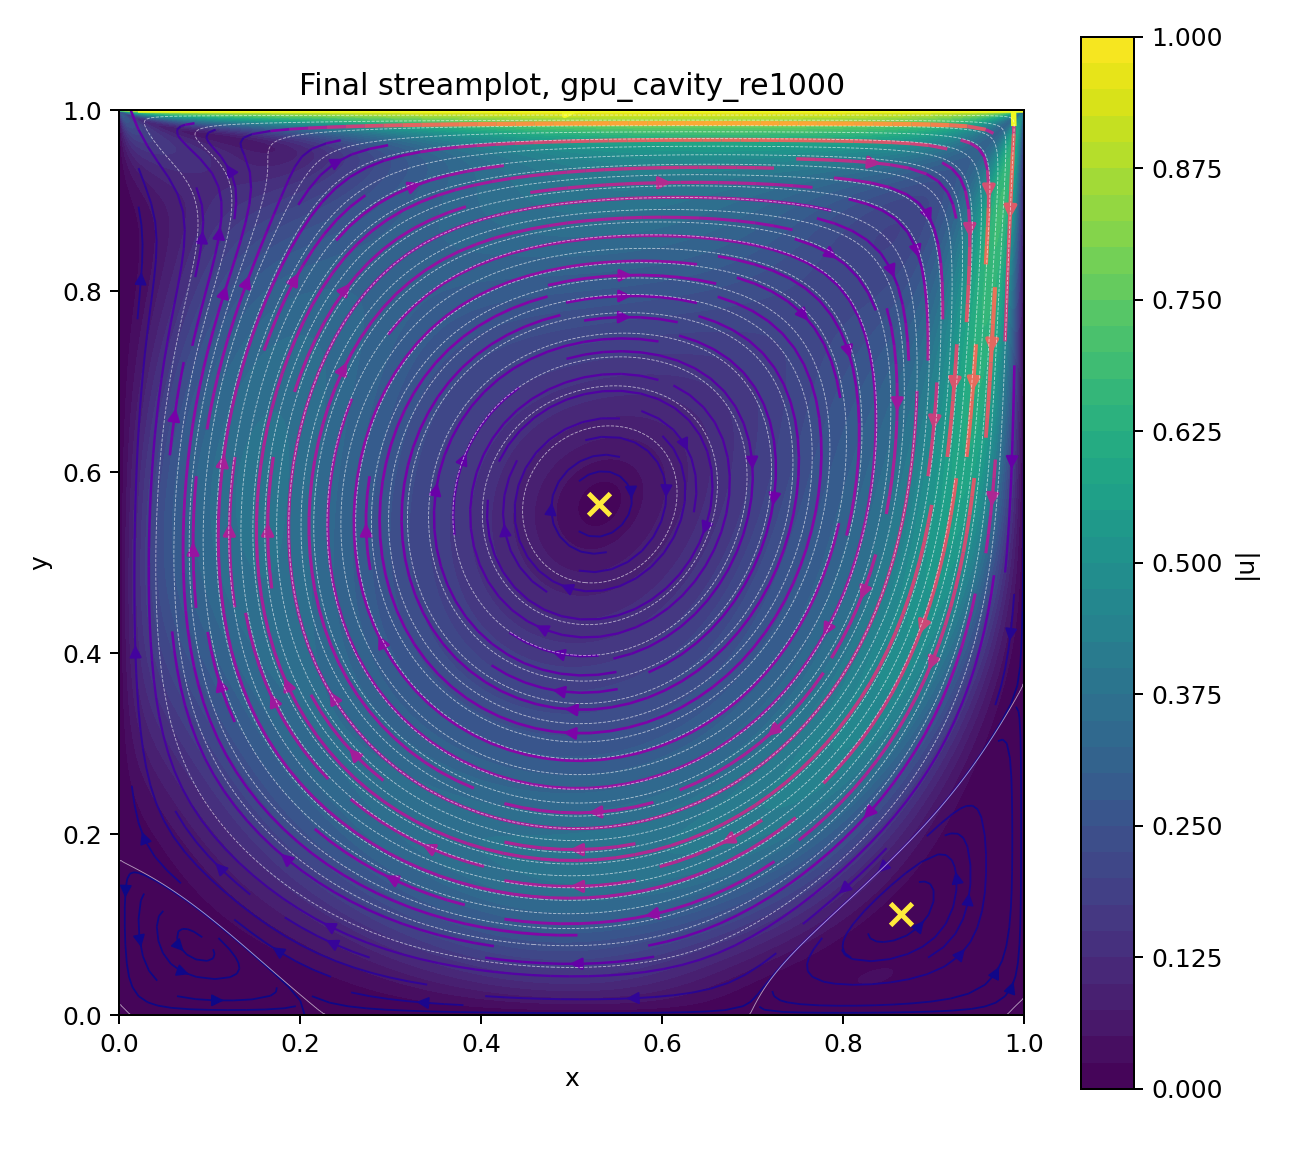
\includegraphics[width=\textwidth]{cavity_re1000_streamplot.png}\\
            \small \(\Reynolds=1000\)
        \end{column}
        \begin{column}{0.32\textwidth}
            \centering
            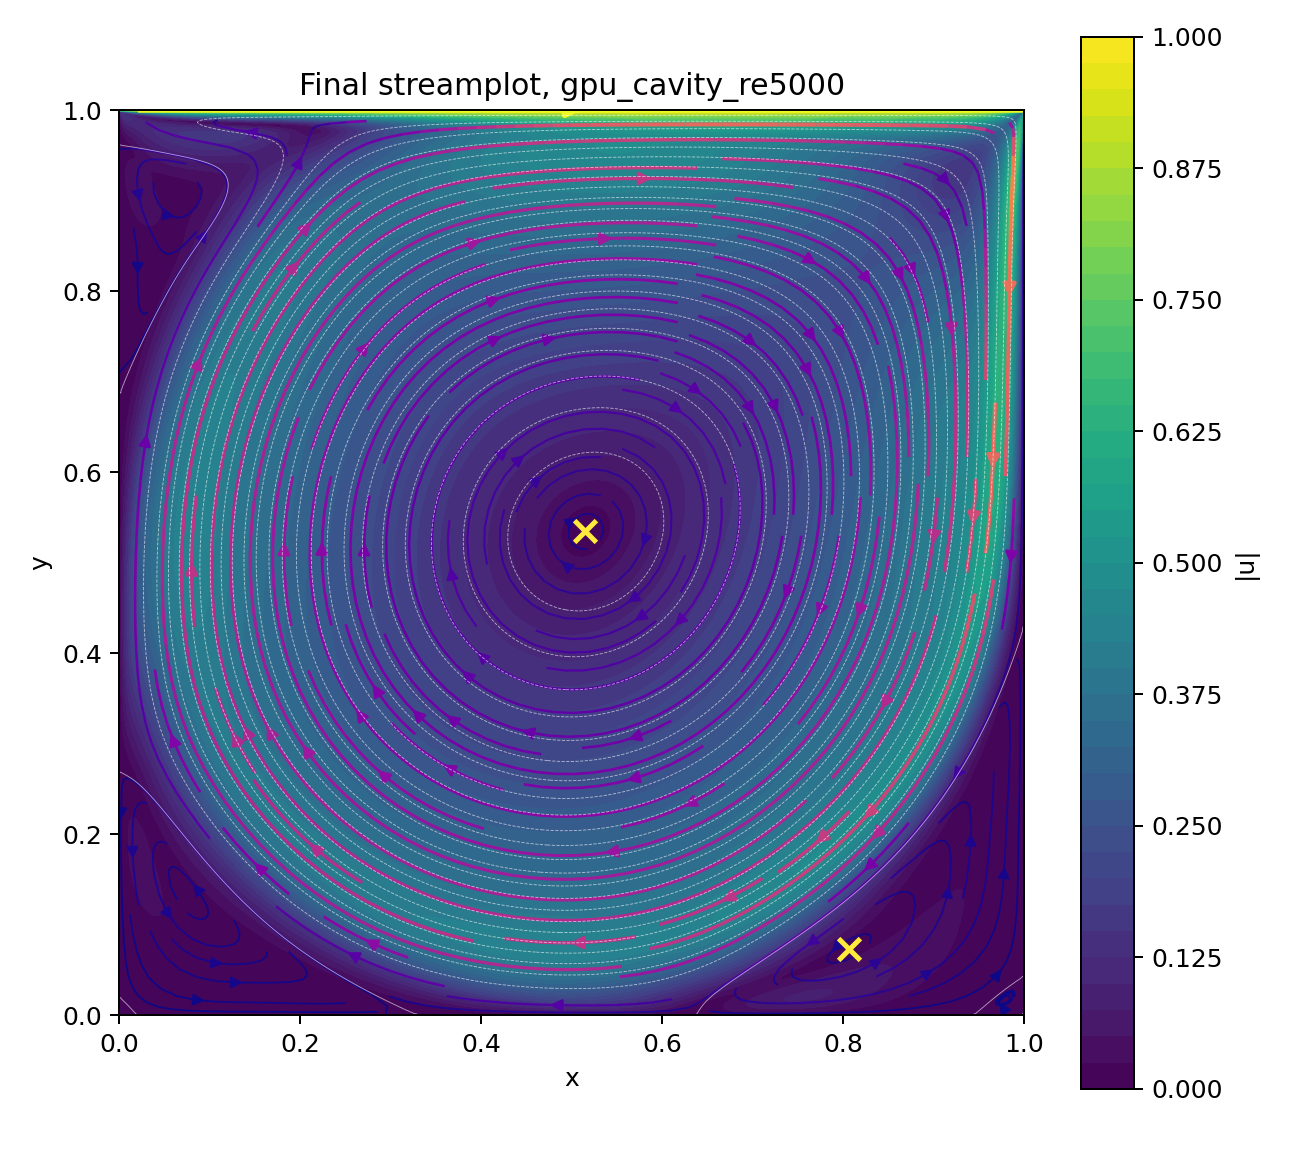
\includegraphics[width=\textwidth]{cavity_re5000_streamplot.png}\\
            \small \(\Reynolds=5000\)
        \end{column}
        \begin{column}{0.32\textwidth}
            \centering
            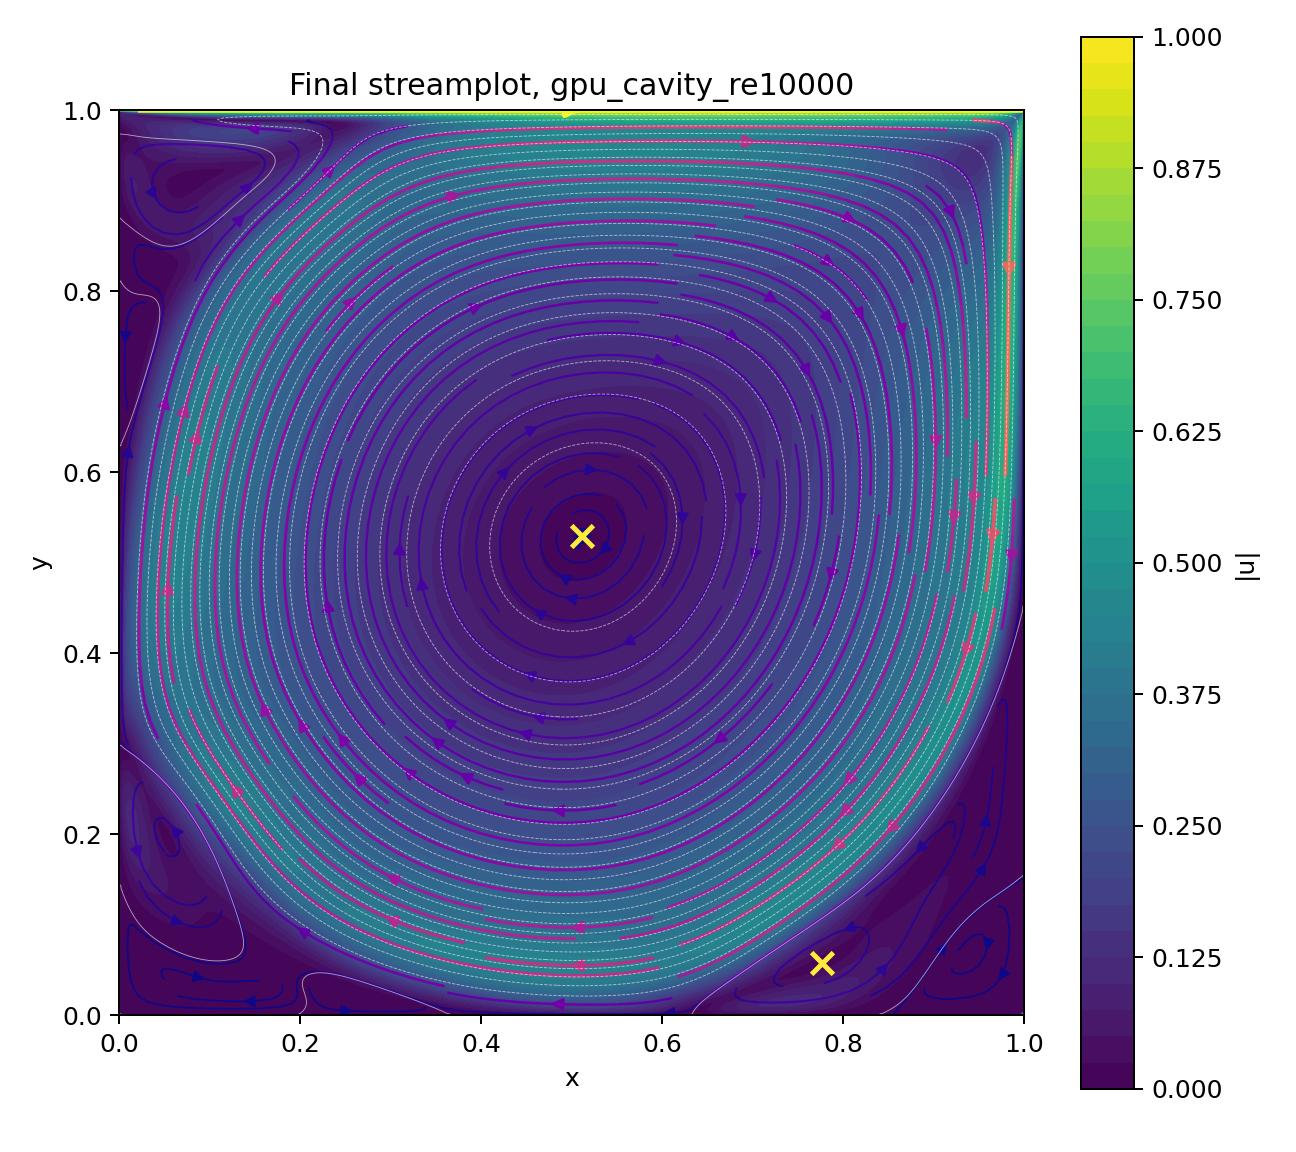
\includegraphics[width=\textwidth]{cavity_re10000_streamplot.png}\\
            \small \(\Reynolds=10000\)
        \end{column}
    \end{columns}
\end{frame}

\begin{frame}{Сравнение центров: \(\Reynolds=1000\)}
    \begin{columns}
        \begin{column}{0.42\textwidth}
            \centering
            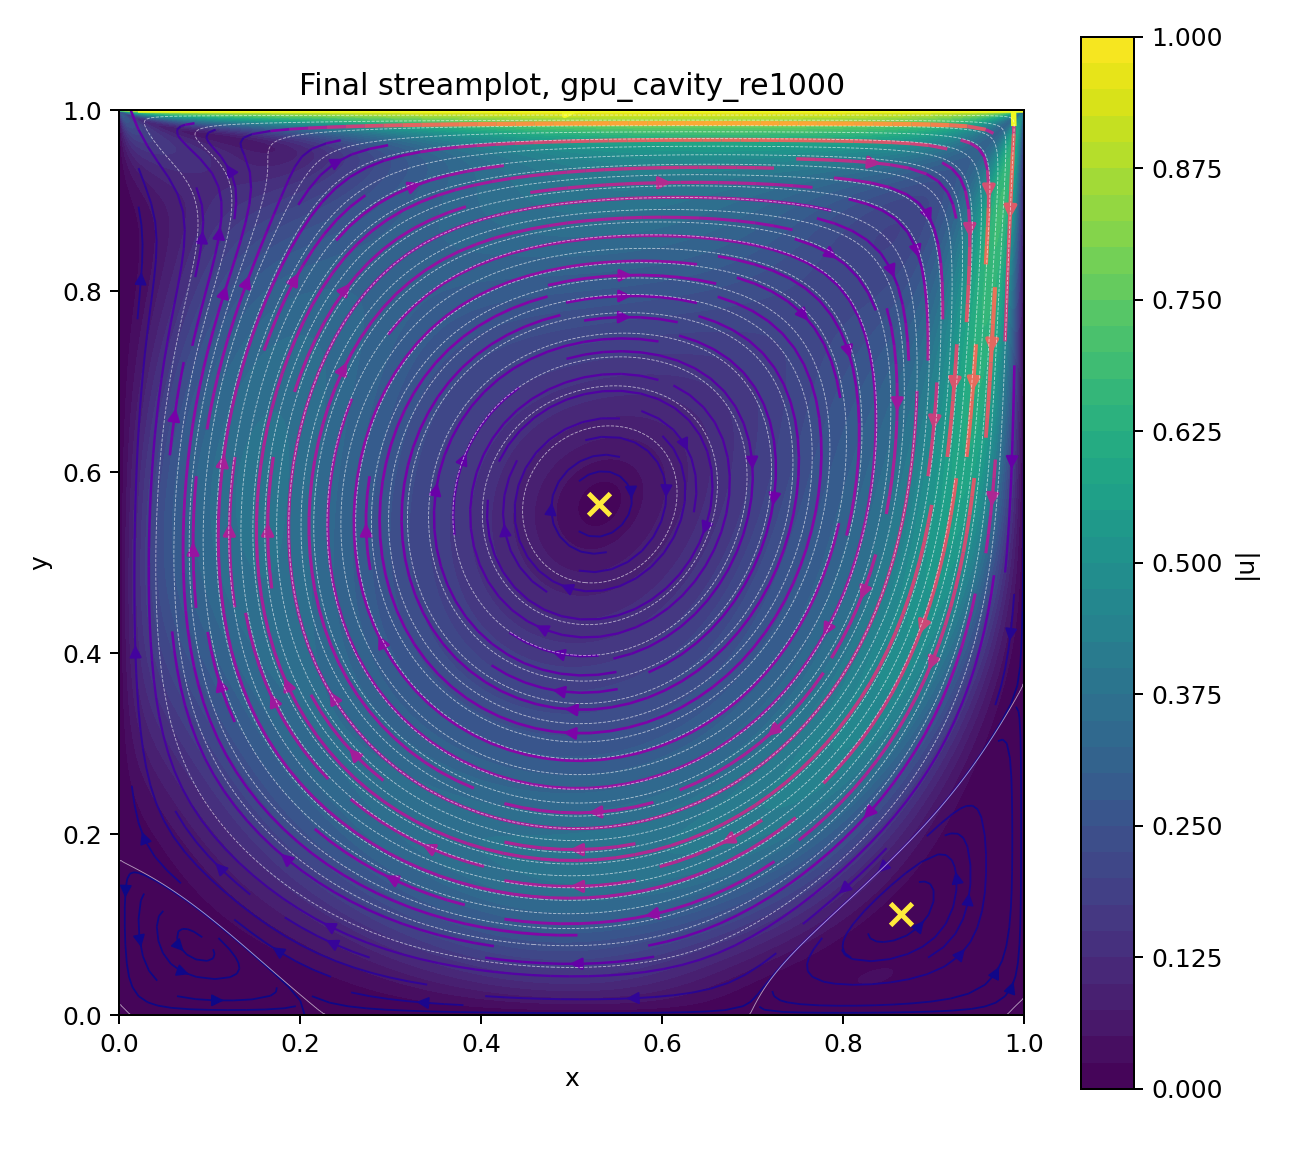
\includegraphics[height=0.36\textheight,keepaspectratio]{cavity_re1000_streamplot.png}\\
            \small расчёт
        \end{column}
        \begin{column}{0.42\textwidth}
            \centering
            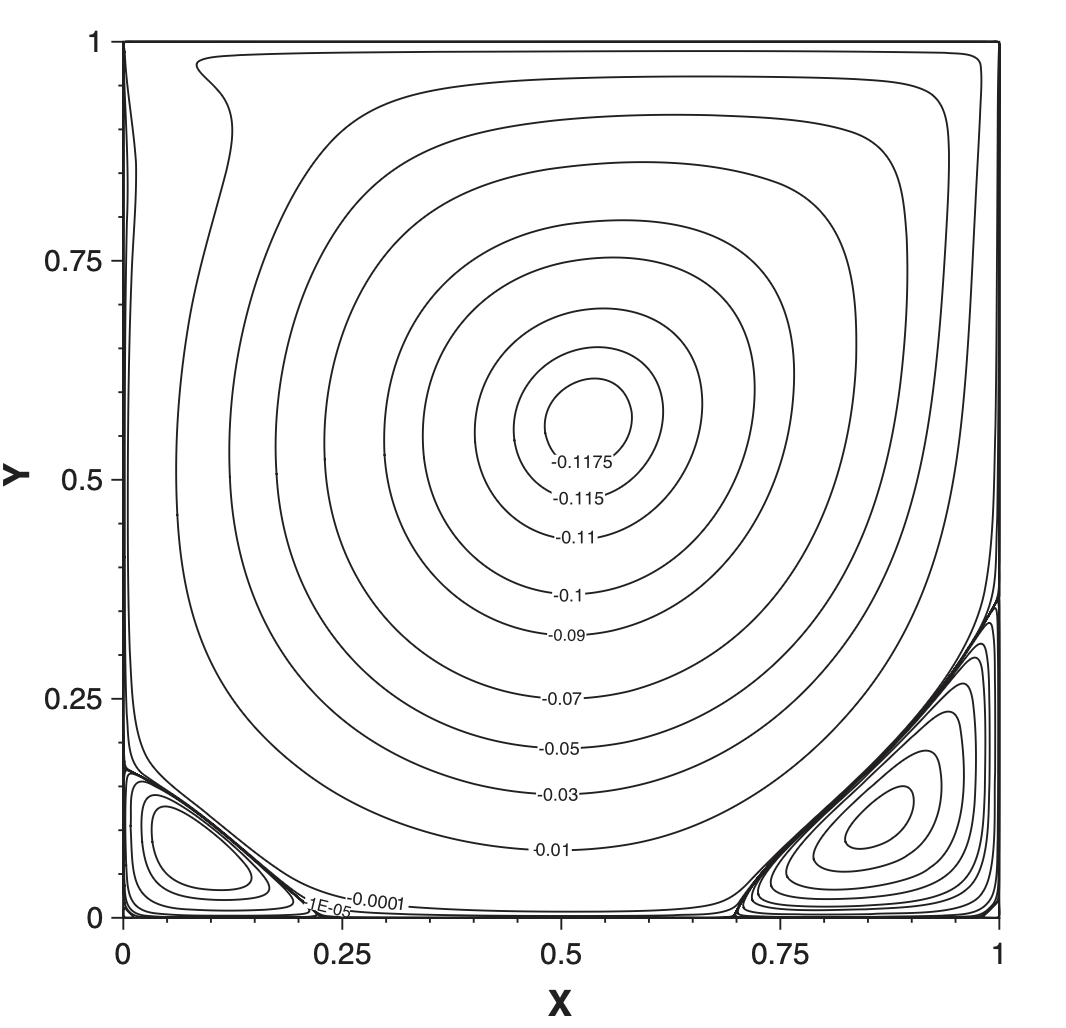
\includegraphics[height=0.36\textheight,keepaspectratio]{images_presentation/paper_1000.png}
        \end{column}
    \end{columns}
    \vspace{0.25em}
    \centering
    \scriptsize
    \resizebox{0.94\textwidth}{!}{%
    \begin{tabular}{lcc}
        \toprule
        Величина & расчёт & Erturk et al.\\
        \midrule
        центр главного вихря & \((0.5300;\ 0.5650)\) & \((0.5300;\ 0.5650)\)\\
        \(\psi\) в главном вихре & \(-0.118781\) & \(-0.118781\)\\
        центр вторичного вихря & \((0.8633;\ 0.1117)\) & \((0.8633;\ 0.1117)\)\\
        \bottomrule
    \end{tabular}
    }
\end{frame}

\begin{frame}{Сравнение центров: \(\Reynolds=5000\)}
    \begin{columns}
        \begin{column}{0.42\textwidth}
            \centering
            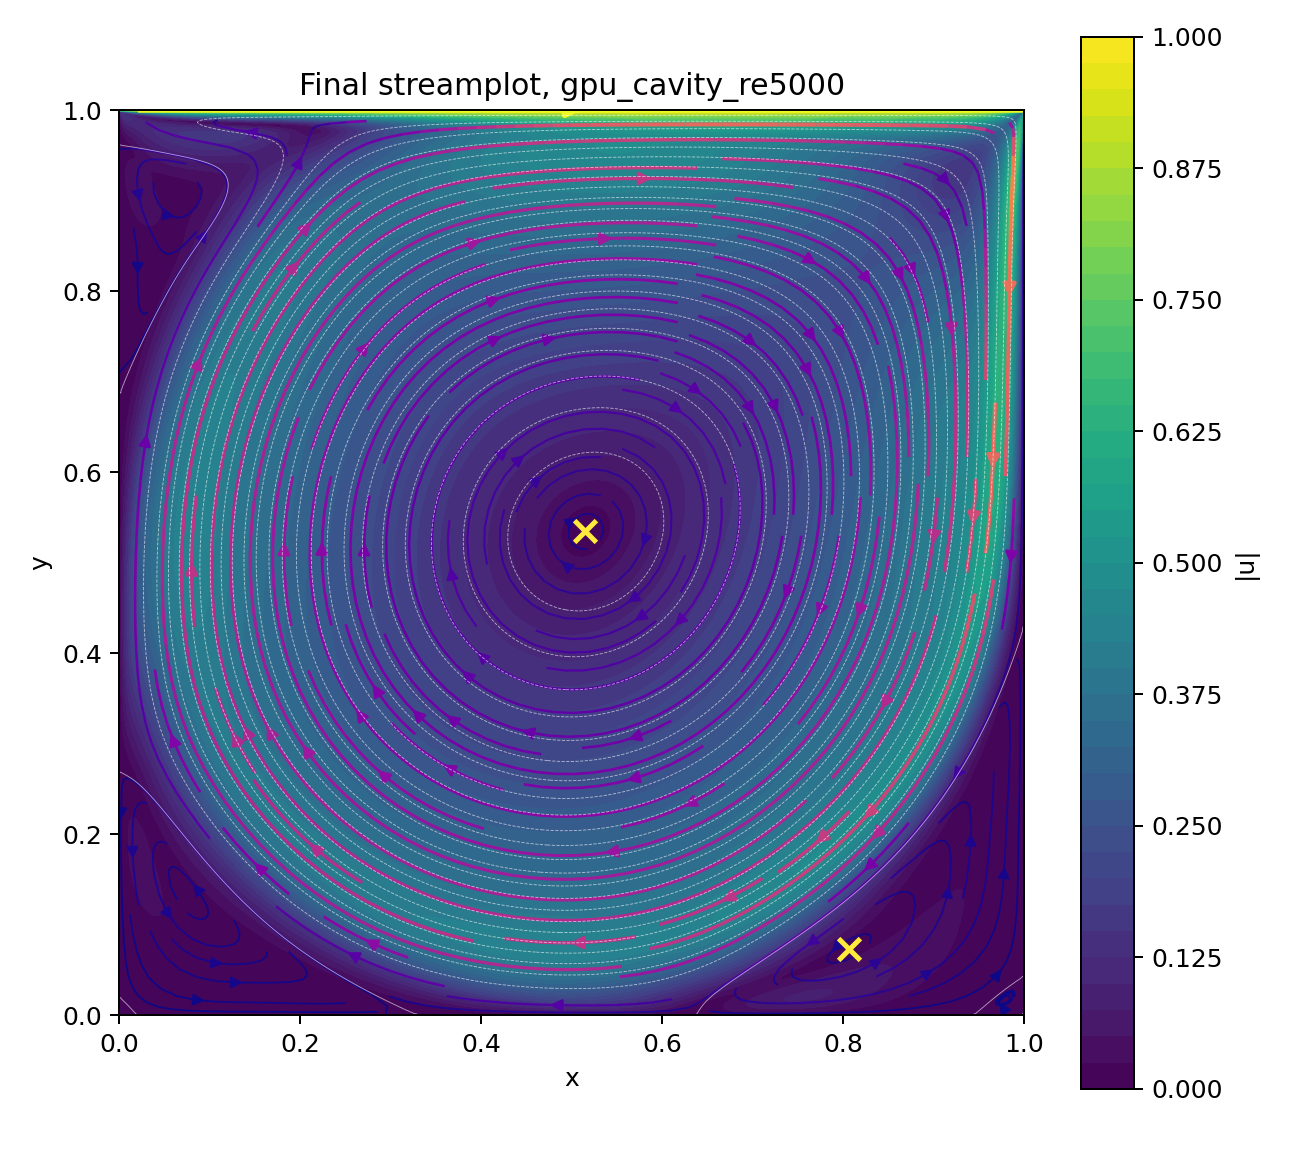
\includegraphics[height=0.36\textheight,keepaspectratio]{cavity_re5000_streamplot.png}\\
            \small расчёт
        \end{column}
        \begin{column}{0.42\textwidth}
            \centering
            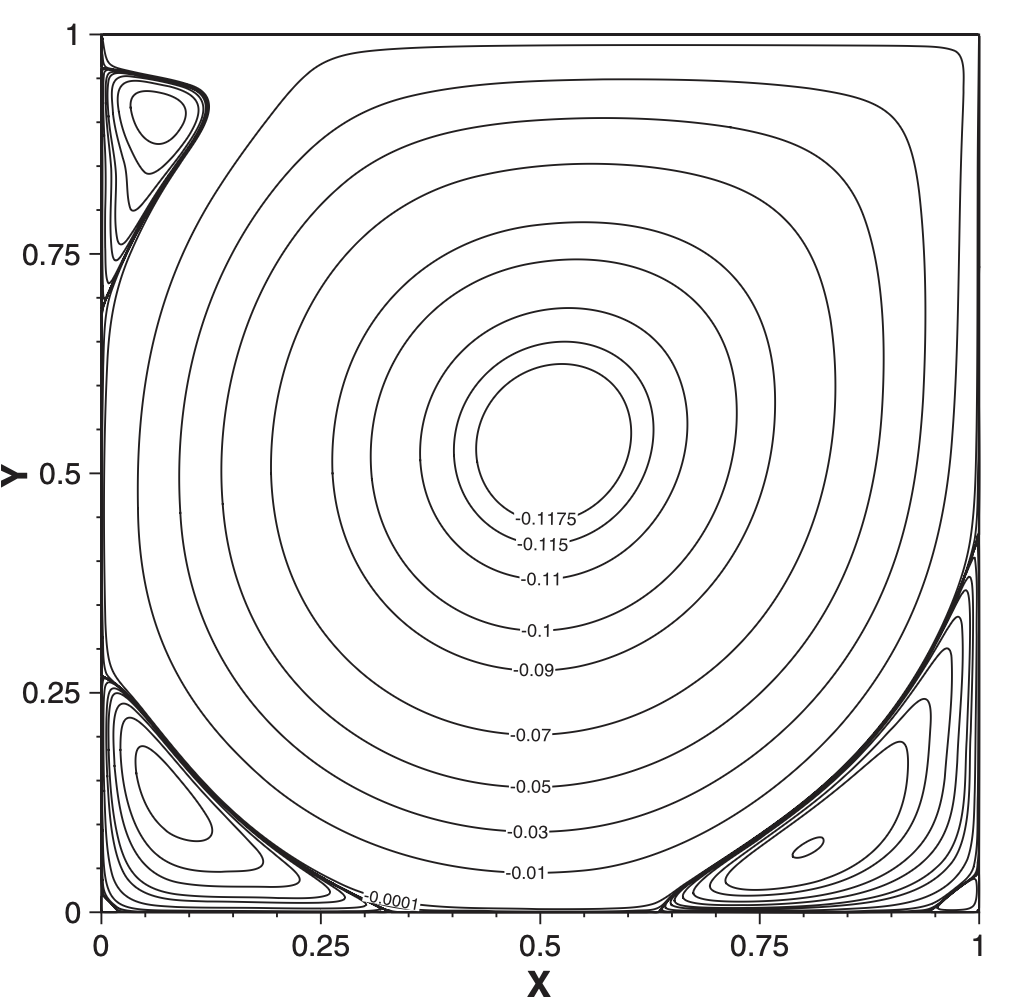
\includegraphics[height=0.36\textheight,keepaspectratio]{images_presentation/paper_5000.png}
        \end{column}
    \end{columns}
    \vspace{0.25em}
    \centering
    \scriptsize
    \resizebox{0.94\textwidth}{!}{%
    \begin{tabular}{lcc}
        \toprule
        Величина & расчёт & Erturk et al.\\
        \midrule
        центр главного вихря & \((0.5150;\ 0.5350)\) & \((0.5150;\ 0.5350)\)\\
        \(\psi\) в главном вихре & \(-0.118382\) & \(-0.121289\)\\
        центр вторичного вихря & \((0.8067;\ 0.0733)\) & \((0.8050;\ 0.0733)\)\\
        \bottomrule
    \end{tabular}
    }
\end{frame}

\begin{frame}{Сравнение центров: \(\Reynolds=10000\)}
    \begin{columns}
        \begin{column}{0.42\textwidth}
            \centering
            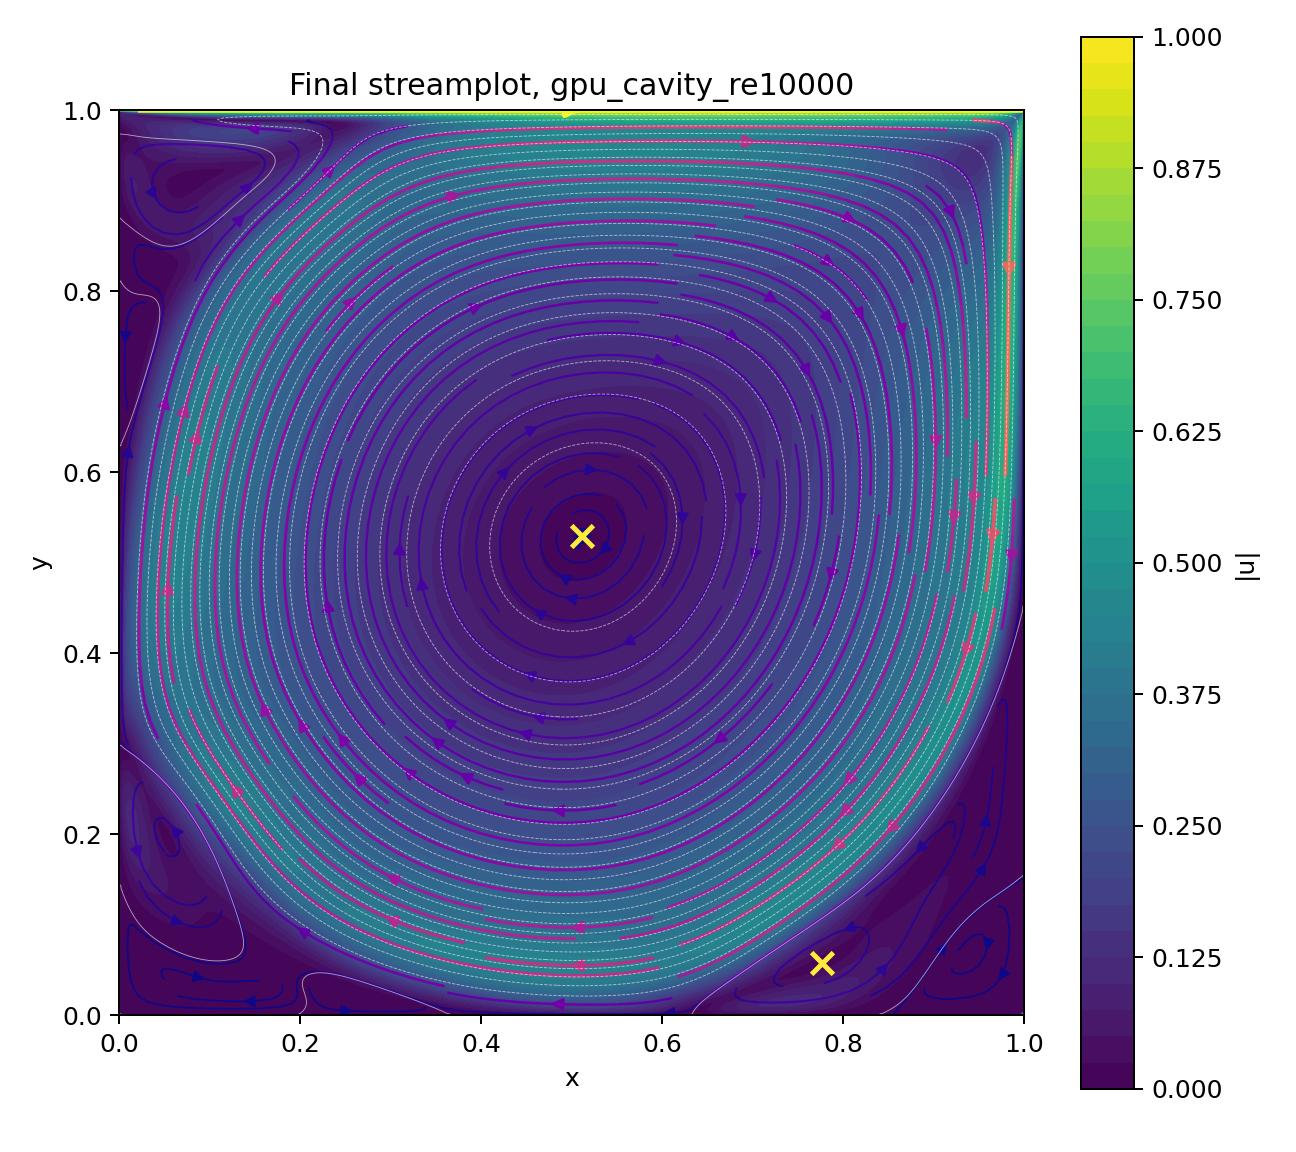
\includegraphics[height=0.36\textheight,keepaspectratio]{cavity_re10000_streamplot.png}\\
            \small расчёт
        \end{column}
        \begin{column}{0.42\textwidth}
            \centering
            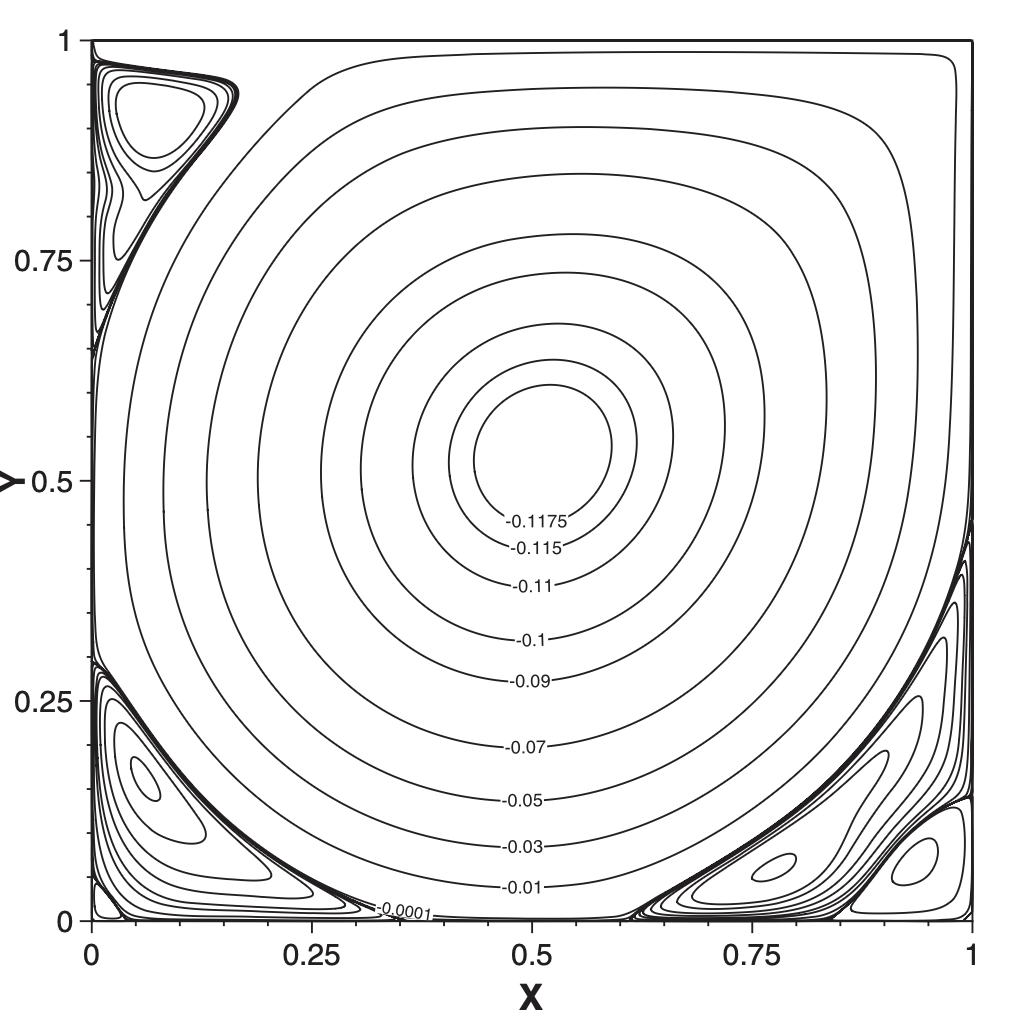
\includegraphics[height=0.36\textheight,keepaspectratio]{images_presentation/paper_10000.png}
        \end{column}
    \end{columns}
    \vspace{0.25em}
    \centering
    \scriptsize
    \resizebox{0.94\textwidth}{!}{%
    \begin{tabular}{lcc}
        \toprule
        Величина & расчёт & Erturk et al.\\
        \midrule
        центр главного вихря & \((0.5117;\ 0.5300)\) & \((0.5117;\ 0.5300)\)\\
        \(\psi\) в главном вихре & \(-0.098797\) & \(-0.120403\)\\
        центр вторичного вихря & \((0.7767;\ 0.0583)\) & \((0.7767;\ 0.0600)\)\\
        \bottomrule
    \end{tabular}
    }
\end{frame}

\begin{frame}{Профили скоростей в каверне}
    \begin{columns}
        \begin{column}{0.32\textwidth}
            \centering
            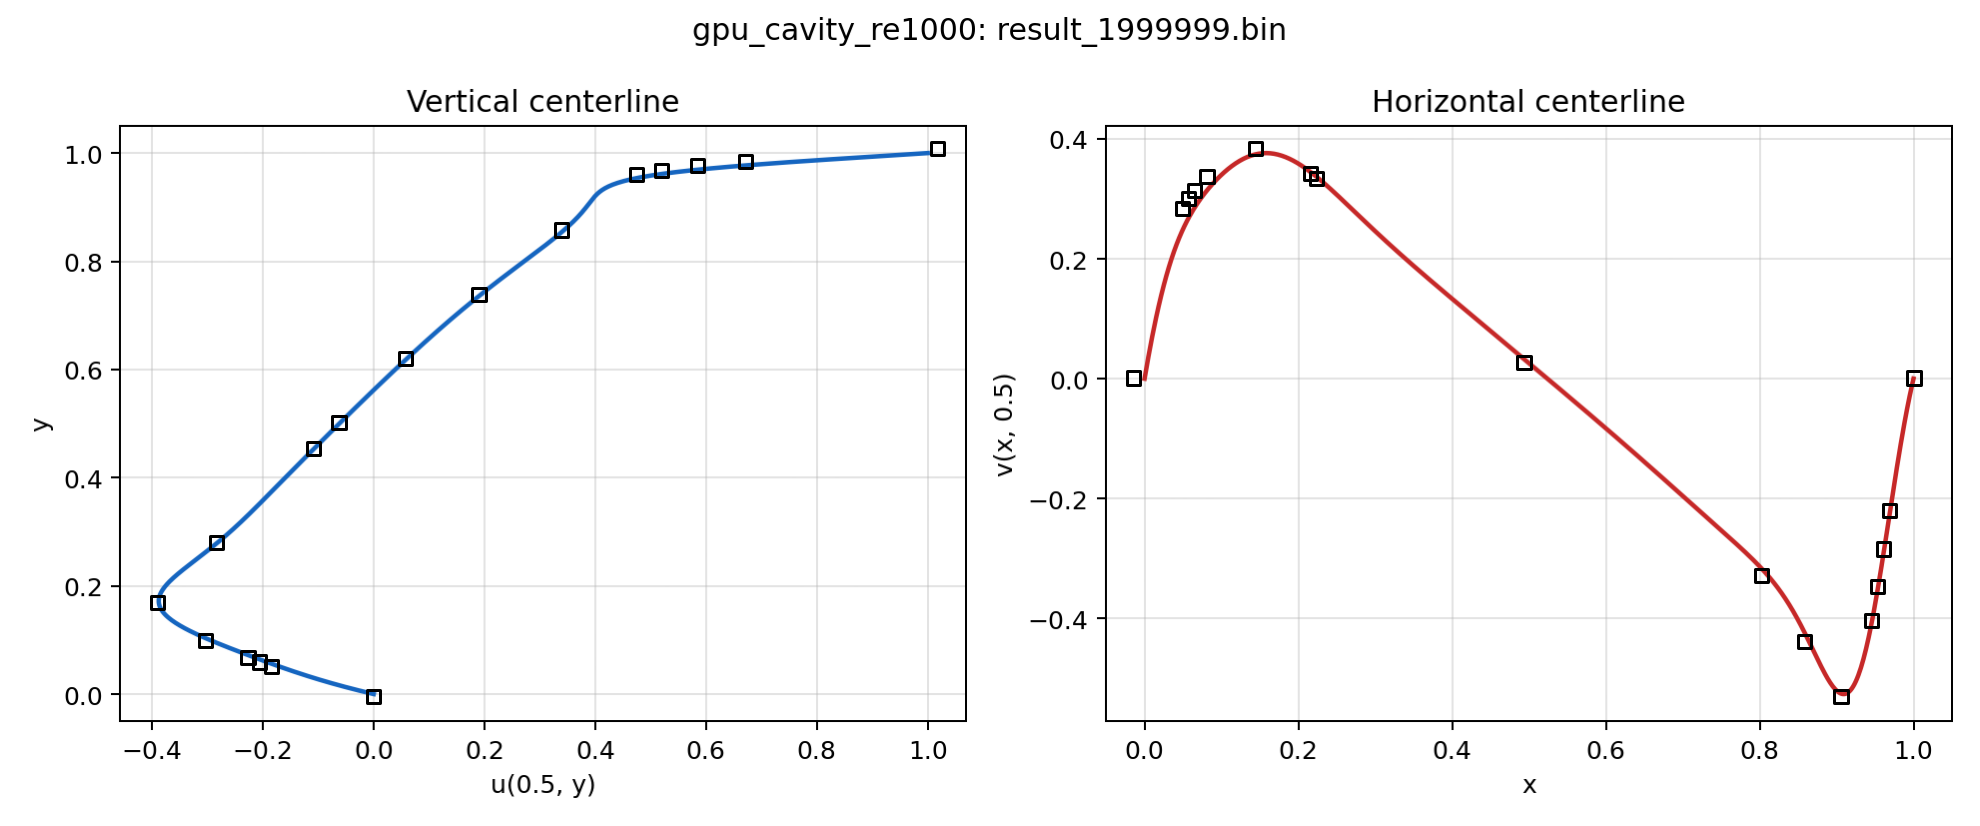
\includegraphics[width=\textwidth]{cavity_re1000_profiles_with_points.png}\\
            \small \(\Reynolds=1000\)
        \end{column}
        \begin{column}{0.32\textwidth}
            \centering
            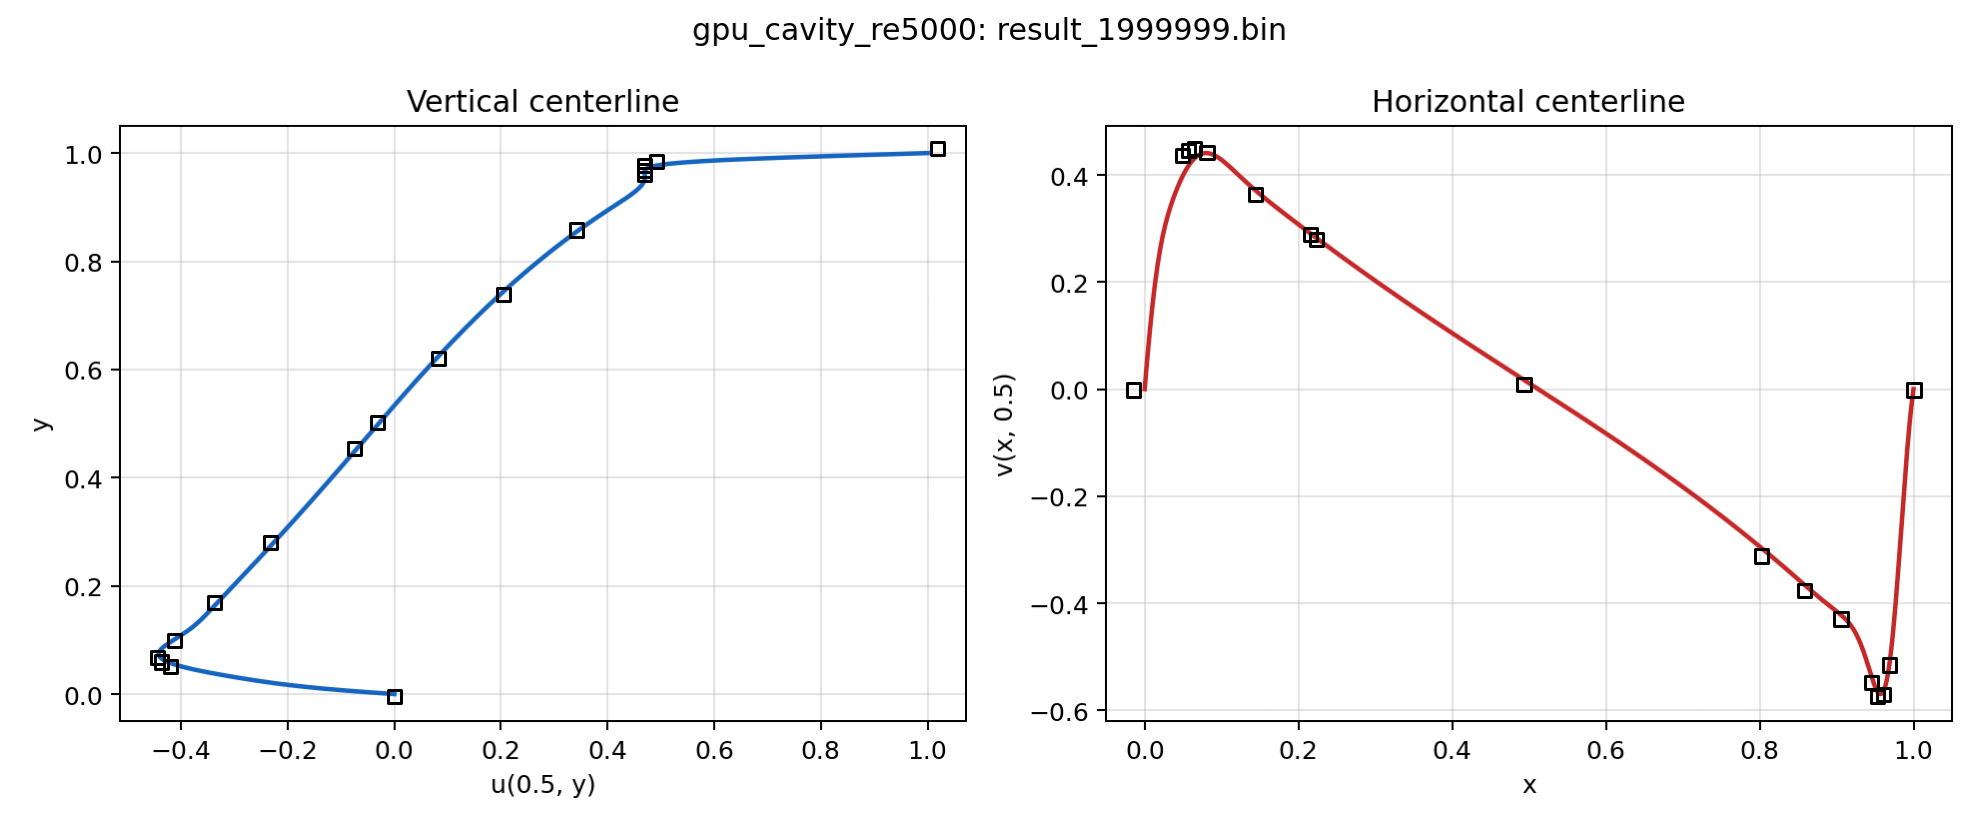
\includegraphics[width=\textwidth]{cavity_re5000_profiles_with_points.png}\\
            \small \(\Reynolds=5000\)
        \end{column}
        \begin{column}{0.32\textwidth}
            \centering
            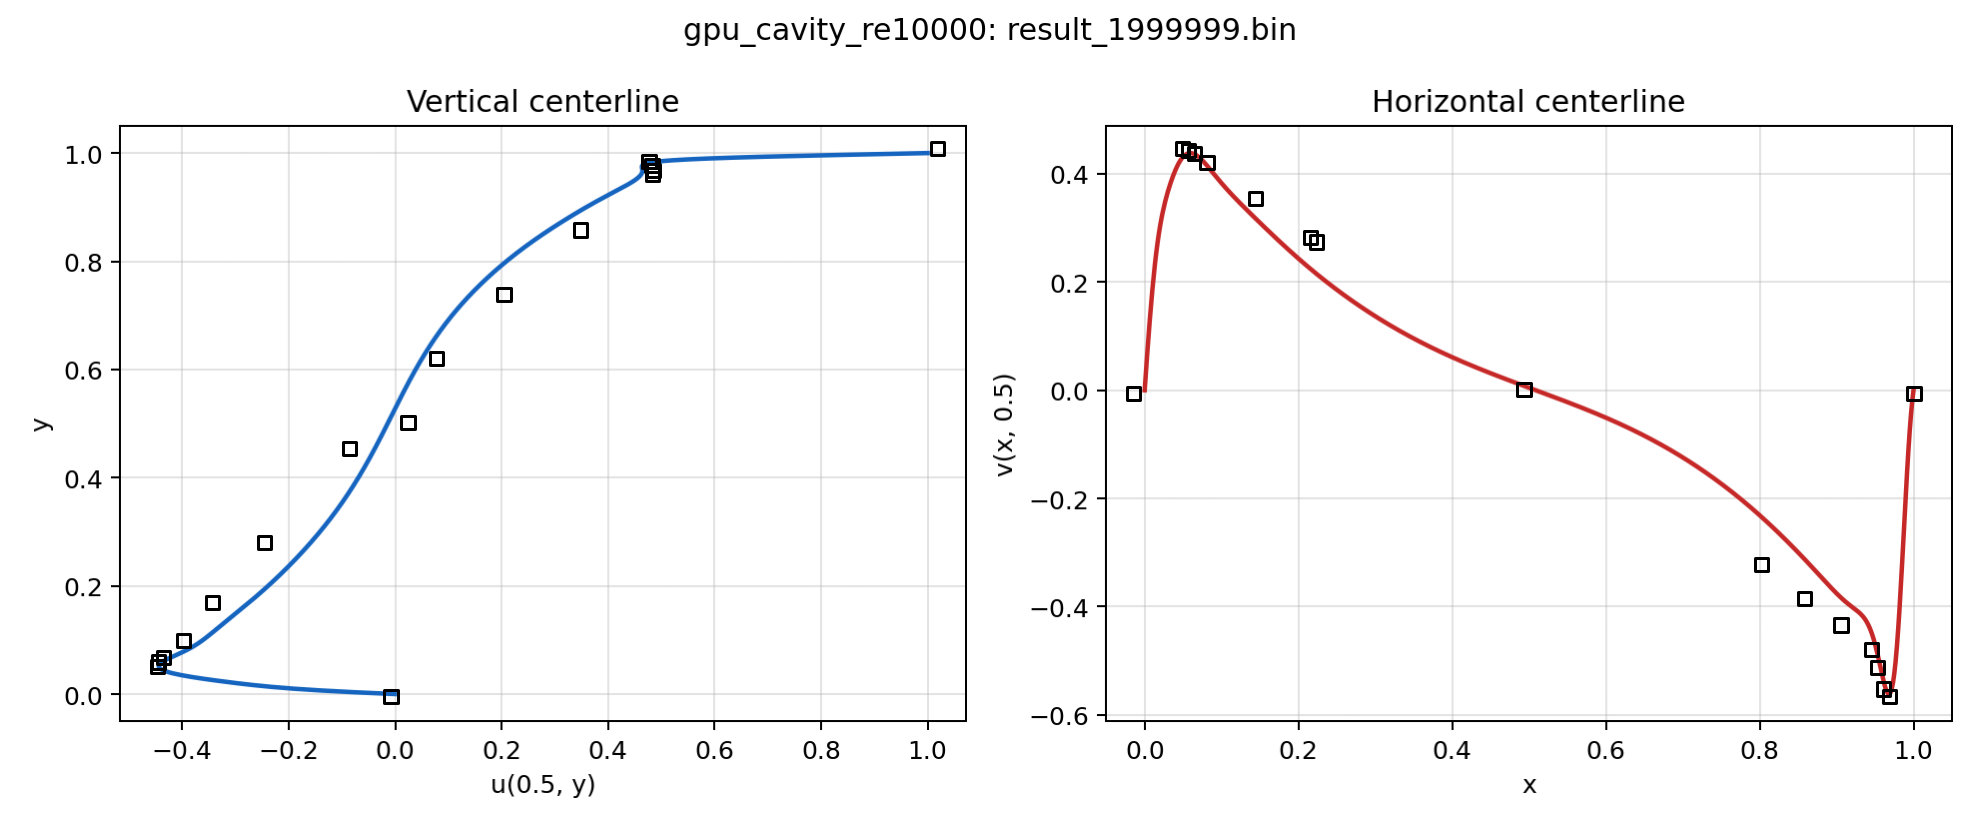
\includegraphics[width=\textwidth]{cavity_re10000_profiles_with_points.png}\\
            \small \(\Reynolds=10000\)
        \end{column}
    \end{columns}
    \vspace{0.3em}
    \centering
    \small Квадратные маркеры --- табличные точки Ghia et al. для центральных профилей скорости.
\end{frame}

\begin{frame}{Стационарная задача и стабилизация}
    Стационарное состояние \(U_*=(\psi_*,\omega_*)\):
    \[
        \Laplace\psi_*+\omega_*=0,
    \]
    \[
        \nu\Laplace\omega_*-\J(\psi_*,\omega_*)-F_\omega(x,y)=0.
    \]
    Линеаризация около стационара:
    \[
        U=U_*+\eta,\qquad
        \dot\eta=\mathcal A\eta,\qquad
        \mathcal A\varphi=\lambda\varphi.
    \]
    Если \(\operatorname{Re}\lambda>0\), соответствующая компонента возмущения растёт.
    Цель стабилизационного эксперимента --- выделить и удалить растущую компоненту.
\end{frame}

\begin{frame}{Четырёхвихревой эксперимент: постановка}
    \begin{columns}
        \begin{column}{0.48\textwidth}
            \[
                \Omega=(0,1)\times(0,0.5),
                \qquad \Reynolds=260.
            \]
            Частные граничные условия:
            \[
                \psi|_{\partial\Omega}=0,\qquad
                U_{\partial\Omega}=0.
            \]
            \[
                F_\omega(x,y)
                =
                \sum_{(m,n)\in\mathcal M}
                a_{mn}\frac{\pi n}{L_y}
                \sin\frac{\pi m x}{L_x}
                \sin\frac{\pi n y}{L_y}.
            \]
        \end{column}
        \begin{column}{0.48\textwidth}
            \centering
            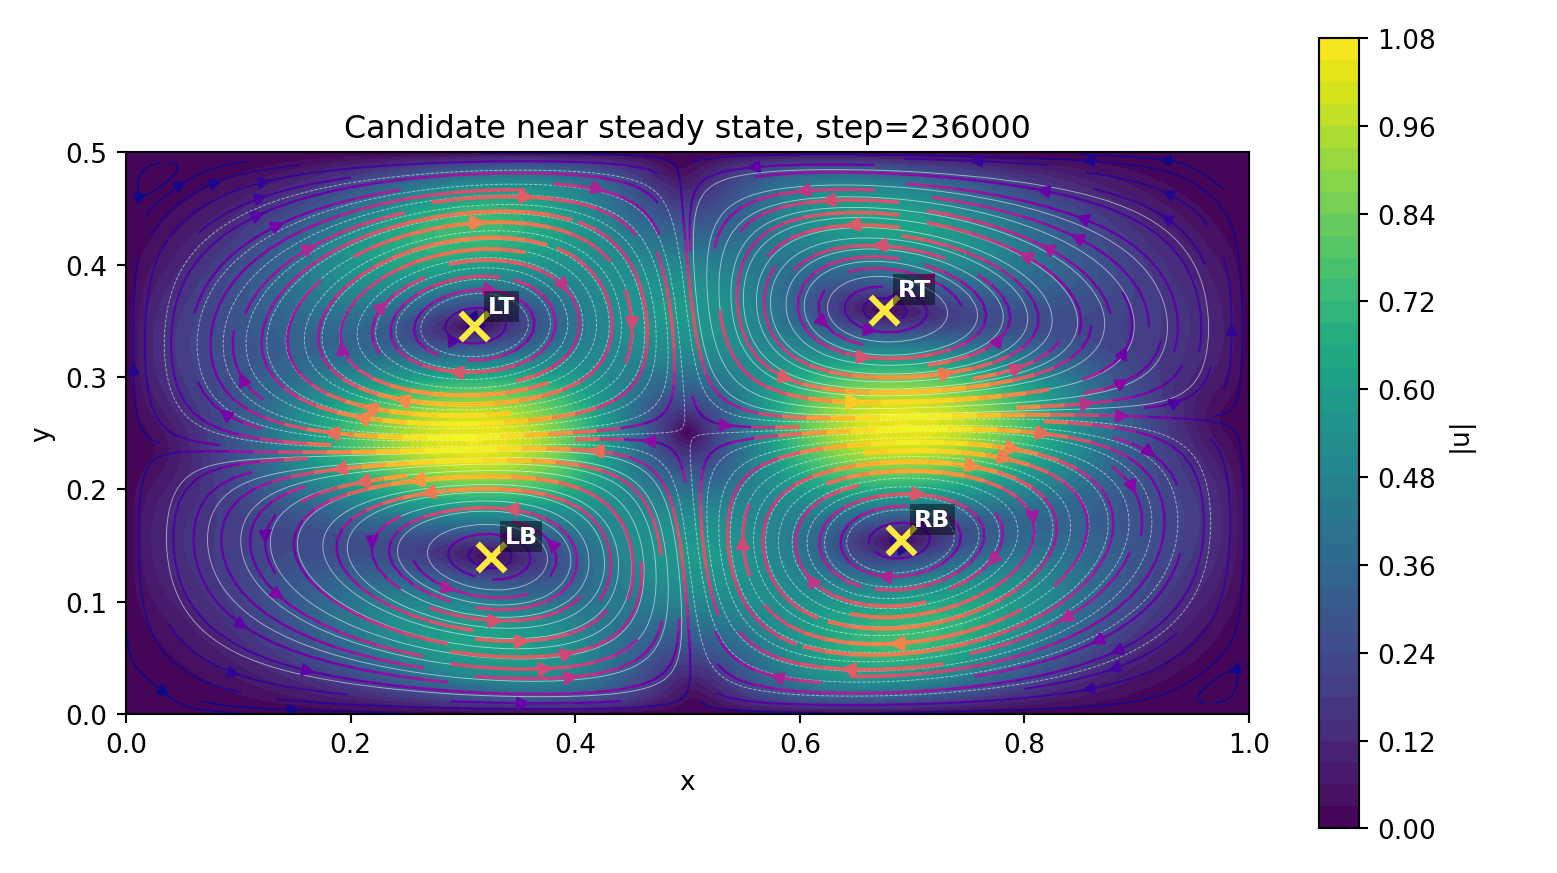
\includegraphics[width=0.92\textwidth]{pulsation_candidate_centers.png}\\
            \small четырёхвихревая структура
        \end{column}
    \end{columns}
\end{frame}

\begin{frame}{Выбор начального приближения}
    \begin{columns}
        \begin{column}{0.50\textwidth}
            Прямое интегрирование из нулевого состояния даёт последовательность сохранённых снимков.

            Кандидат в стационар выбирается как снимок, на котором достигается минимум разности по сохранённым результатам.
            \[
                n=236000,\qquad t=2.36001.
            \]
            Этот снимок используется как начальное приближение для метода Ньютона.
        \end{column}
        \begin{column}{0.46\textwidth}
            \centering
            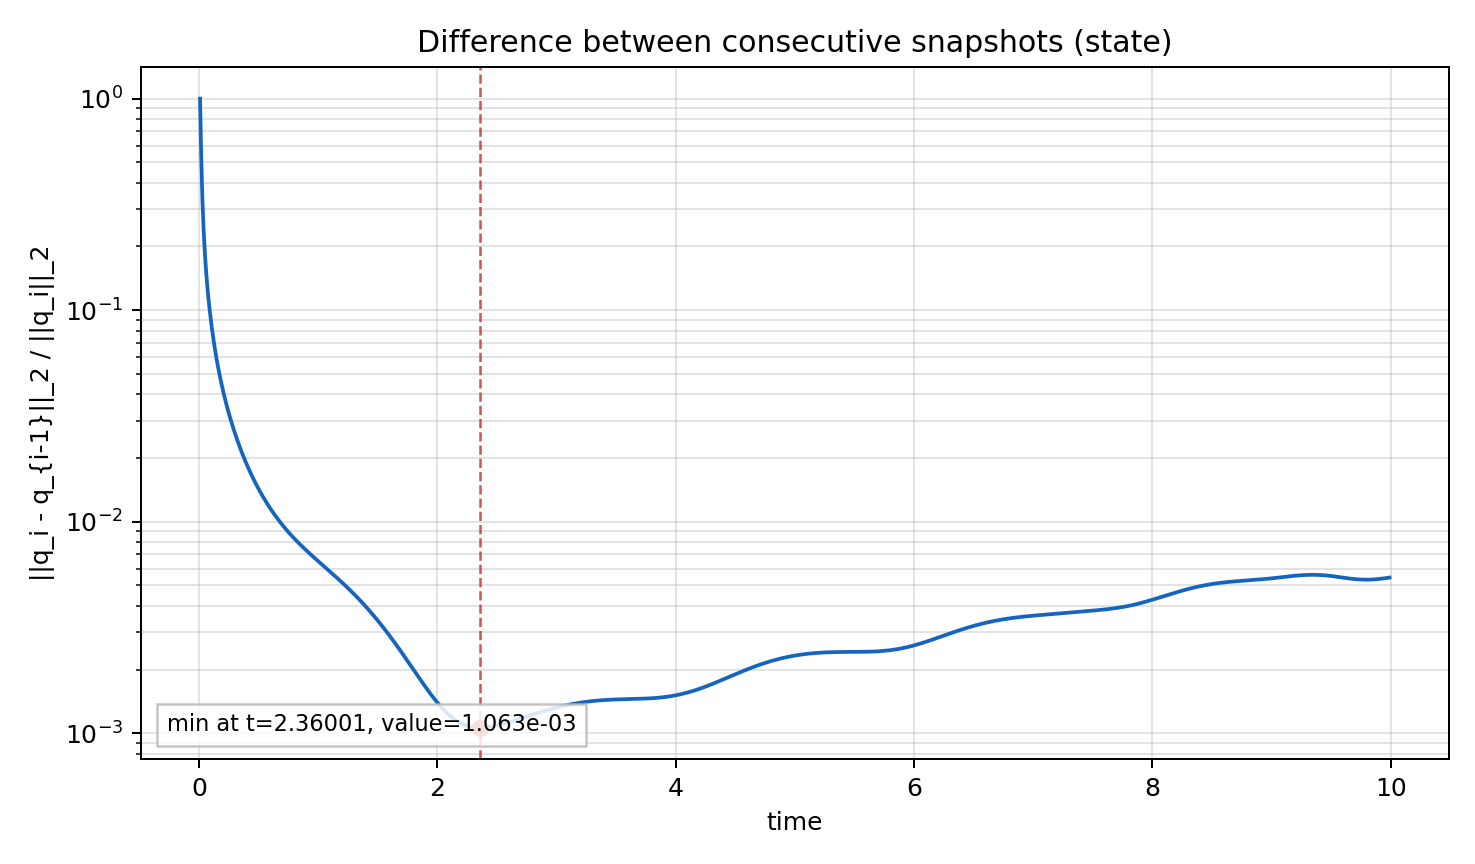
\includegraphics[width=0.95\textwidth]{stationary_consecutive_difference.png}
        \end{column}
    \end{columns}
\end{frame}

\begin{frame}{Прямой расчёт без коррекции}
    \begin{columns}
        \begin{column}{0.48\textwidth}
            \centering
            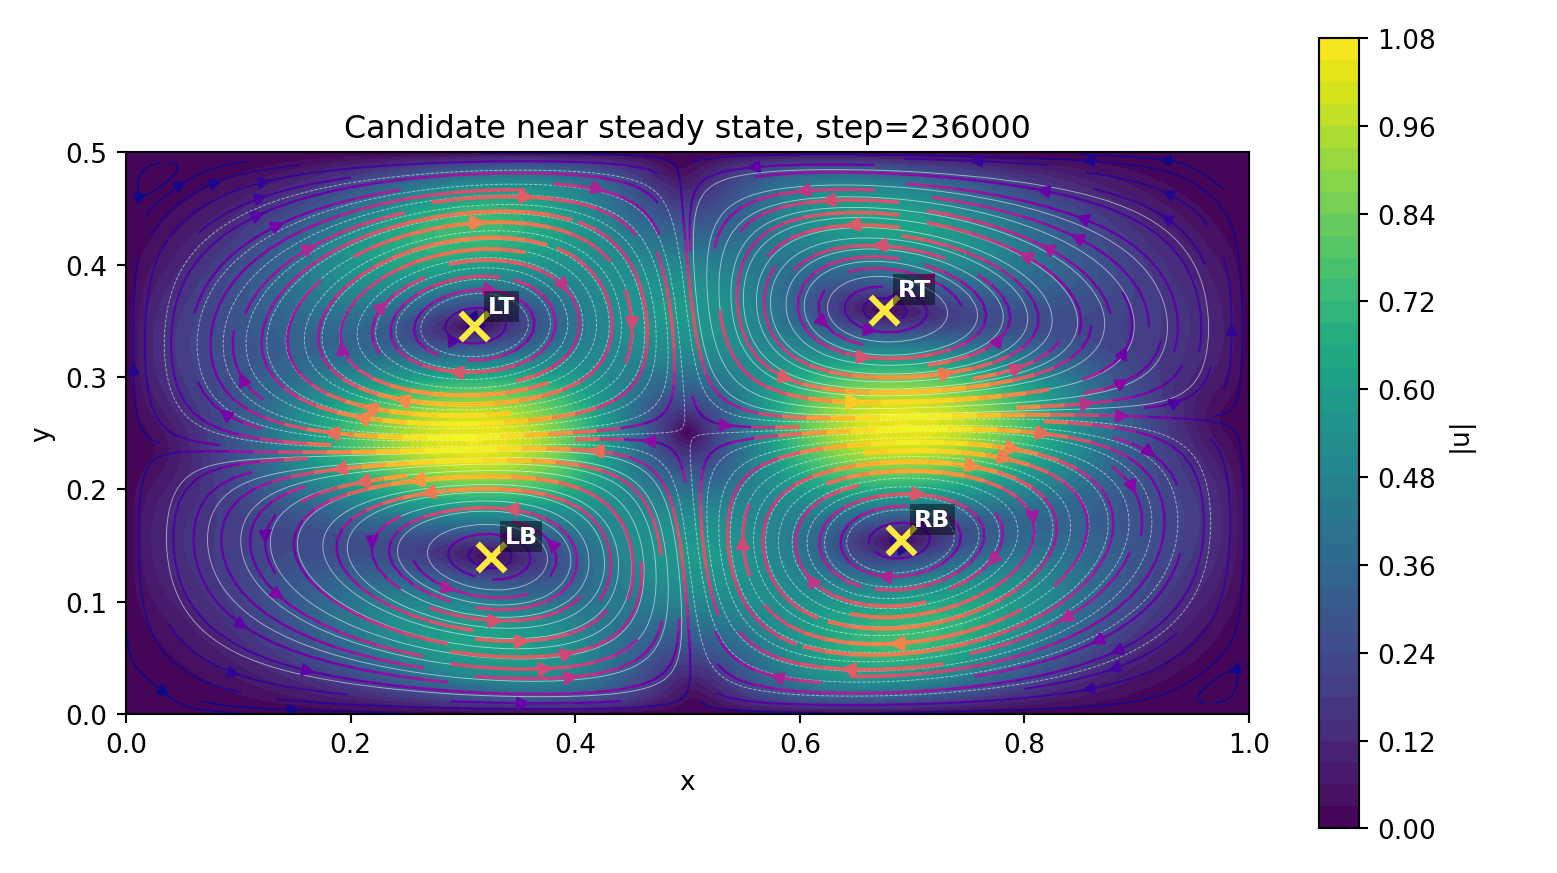
\includegraphics[width=0.92\textwidth]{pulsation_candidate_centers.png}\\
            \small кандидат в стационарное состояние
        \end{column}
        \begin{column}{0.48\textwidth}
            \centering
            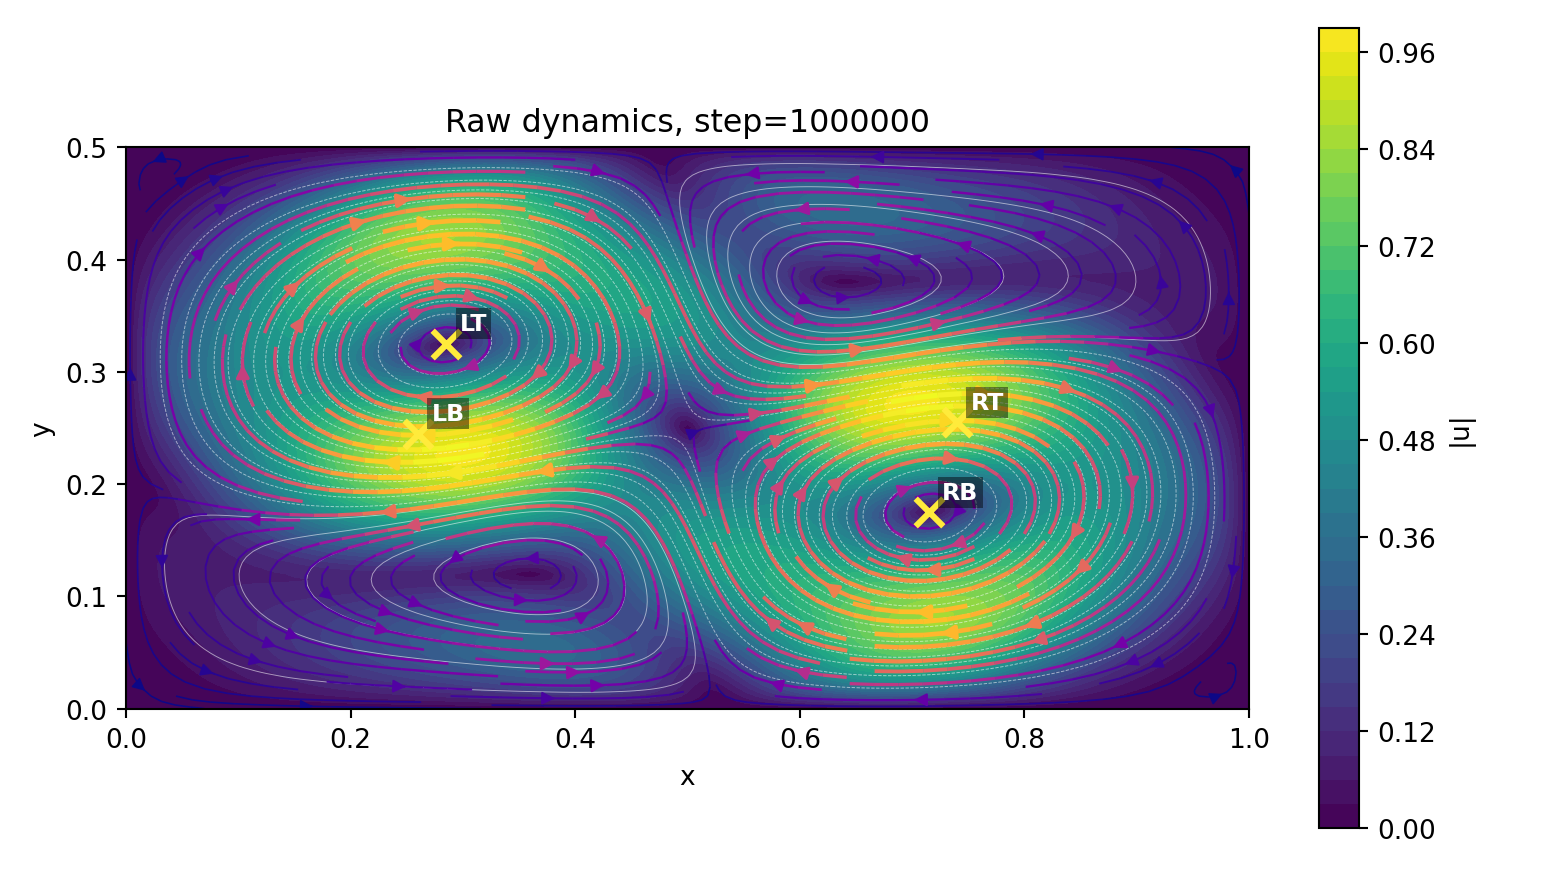
\includegraphics[width=0.92\textwidth]{pulsation_raw_1000000_centers.png}\\
            \small прямой расчёт, шаг \(10^6\)
        \end{column}
    \end{columns}
    \vspace{0.3em}
    \centering
    \small При продолжении прямого интегрирования решение уходит от четырёхвихревой структуры; это мотивирует спектральный анализ около стационара.
\end{frame}

\begin{frame}{Метод Ньютона для стационара}
    Дискретная стационарная система записывается как
    \[
        F(U)=0,\qquad
        U=(\psi,\omega)^T.
    \]
    На \(k\)-й итерации решается линейная система для поправки:
    \[
        F'(U_k)\delta U_k=-F(U_k).
    \]
    После этого выполняется обновление:
    \[
        U_{k+1}=U_k+\alpha_k\delta U_k,
        \qquad
        0<\alpha_k\le 1.
    \]
    Параметр \(\alpha_k\) выбирается поиском по шагу так, чтобы уменьшалась норма невязки.
    Линейная система решается методом GMRES с матрично-свободным действием якобиана.
\end{frame}

\begin{frame}{Уточнённый стационар}
    \begin{columns}
        \begin{column}{0.48\textwidth}
            \centering
            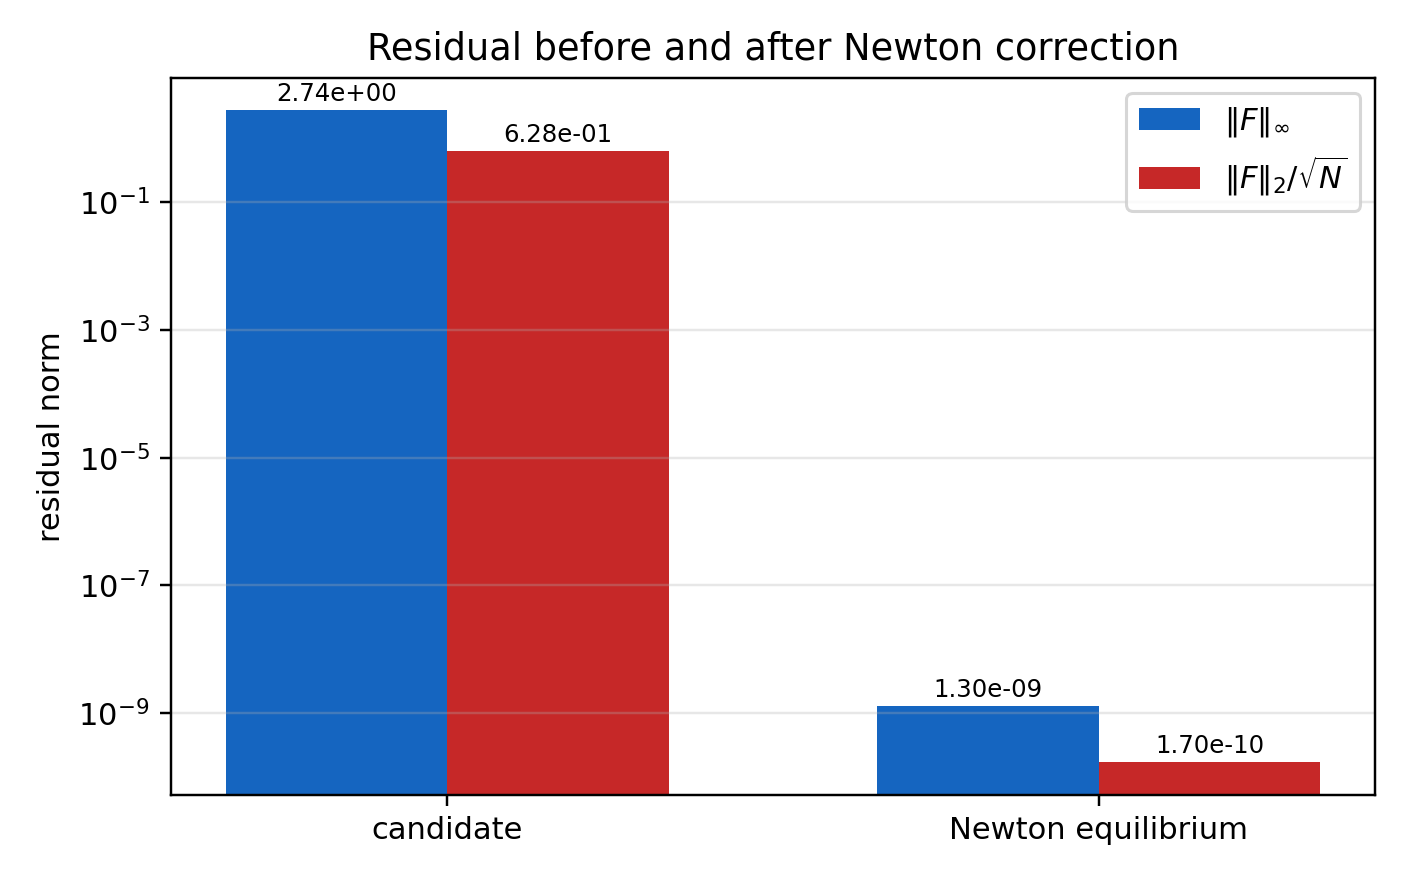
\includegraphics[width=0.95\textwidth]{newton_residual_drop.png}\\
            \small убывание невязки Ньютона
        \end{column}
        \begin{column}{0.48\textwidth}
            \centering
            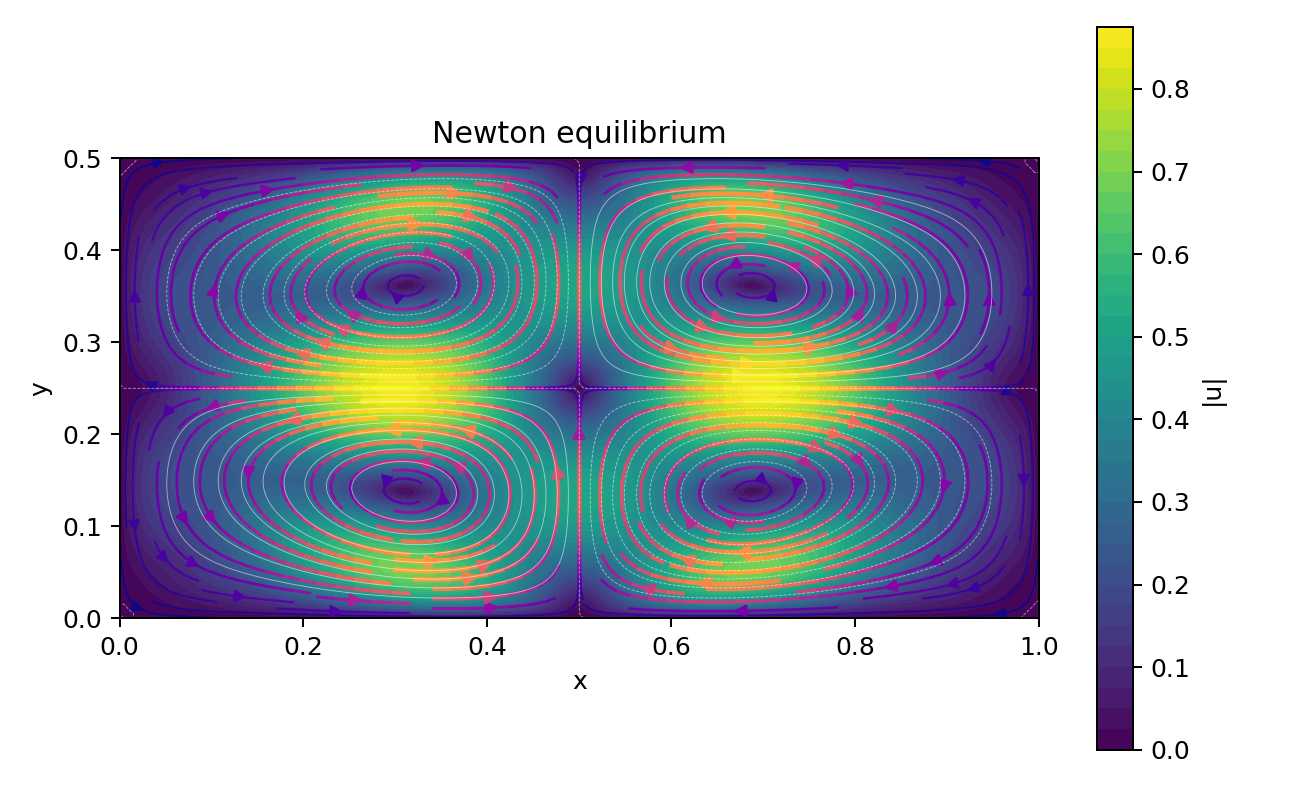
\includegraphics[width=0.95\textwidth]{newton_equilibrium_streamplot.png}\\
            \small стационар после уточнения
        \end{column}
    \end{columns}
\end{frame}

\begin{frame}{Линеаризация: вывод оператора}
    Стационарное состояние обозначается
    \[
        U_*=(\psi_*,\omega_*).
    \]
    Рассматривается малое возмущение:
    \[
        \psi=\psi_*+\phi,\qquad
        \omega=\omega_*+\eta.
    \]
    Стационарная система:
    \[
        \Laplace\psi_*+\omega_*=0,
        \qquad
        \nu\Laplace\omega_*-\J(\psi_*,\omega_*)-F_\omega=0.
    \]
    Линеаризация выполняется так:
    \begin{enumerate}
        \item подставляются \(\psi_*+\phi\) и \(\omega_*+\eta\) в исходную систему;
        \item вычитаются уравнения для стационара;
        \item отбрасываются квадратичные малые члены.
    \end{enumerate}
\end{frame}

\begin{frame}{Спектральная задача: оператор}
    Нелинейный член раскладывается следующим образом:
    \[
        \J(\psi_*+\phi,\omega_*+\eta)
        =
        \J(\psi_*,\omega_*)
        +
        \J(\phi,\omega_*)
        +
        \J(\psi_*,\eta)
        +
        \J(\phi,\eta).
    \]
    Член \(\J(\psi_*,\omega_*)\) сокращается со стационарным уравнением, а \(\J(\phi,\eta)\) является квадратично малым.
    Поэтому остаётся линейная система:
    \[
        \Laplace\phi+\eta=0,
        \qquad
        \eta_t
        =
        \nu\Laplace\eta
        -
        \J(\phi,\omega_*)
        -
        \J(\psi_*,\eta).
    \]
    Из уравнения Пуассона:
    \[
        \phi=-\Laplace^{-1}\eta,
        \qquad
        \phi|_{\partial\Omega}=0.
    \]
    Поэтому
    \[
        \eta_t=\mathcal A\eta.
    \]
\end{frame}

\begin{frame}{Спектральная задача}
    Для нормальной моды
    \[
        \eta(x,y,t)=e^{\lambda t}\varphi(x,y)
    \]
    производная по времени даёт
    \[
        \eta_t=\lambda e^{\lambda t}\varphi.
    \]
    После сокращения общего множителя \(e^{\lambda t}\):
    \[
        \mathcal A\varphi=\lambda\varphi.
    \]
    Здесь
    \[
        \mathcal A\eta
        =
        \nu\Laplace\eta
        -
        \J(-\Laplace^{-1}\eta,\omega_*)
        -
        \J(\psi_*,\eta).
    \]
\end{frame}

\begin{frame}{Спектральная задача: вычисление}
    В дискретной задаче матрица \(\mathcal A_h\) явно не собирается.
    Для действия \(\xi\mapsto\mathcal A_h\xi\) сначала решается задача Пуассона
    \[
        \Laplace_h\chi+\xi=0,
    \]
    затем вычисляется
    \[
        \mathcal A_h\xi
        =
        \nu\Laplace_h\xi
        -
        \J_h(\chi,\omega_*)
        -
        \J_h(\psi_*,\xi).
    \]
    Собственные значения ищутся методом Арнольди.
\end{frame}

\begin{frame}{Спектр и неустойчивая мода}
    \begin{columns}
        \begin{column}{0.45\textwidth}
            \centering
            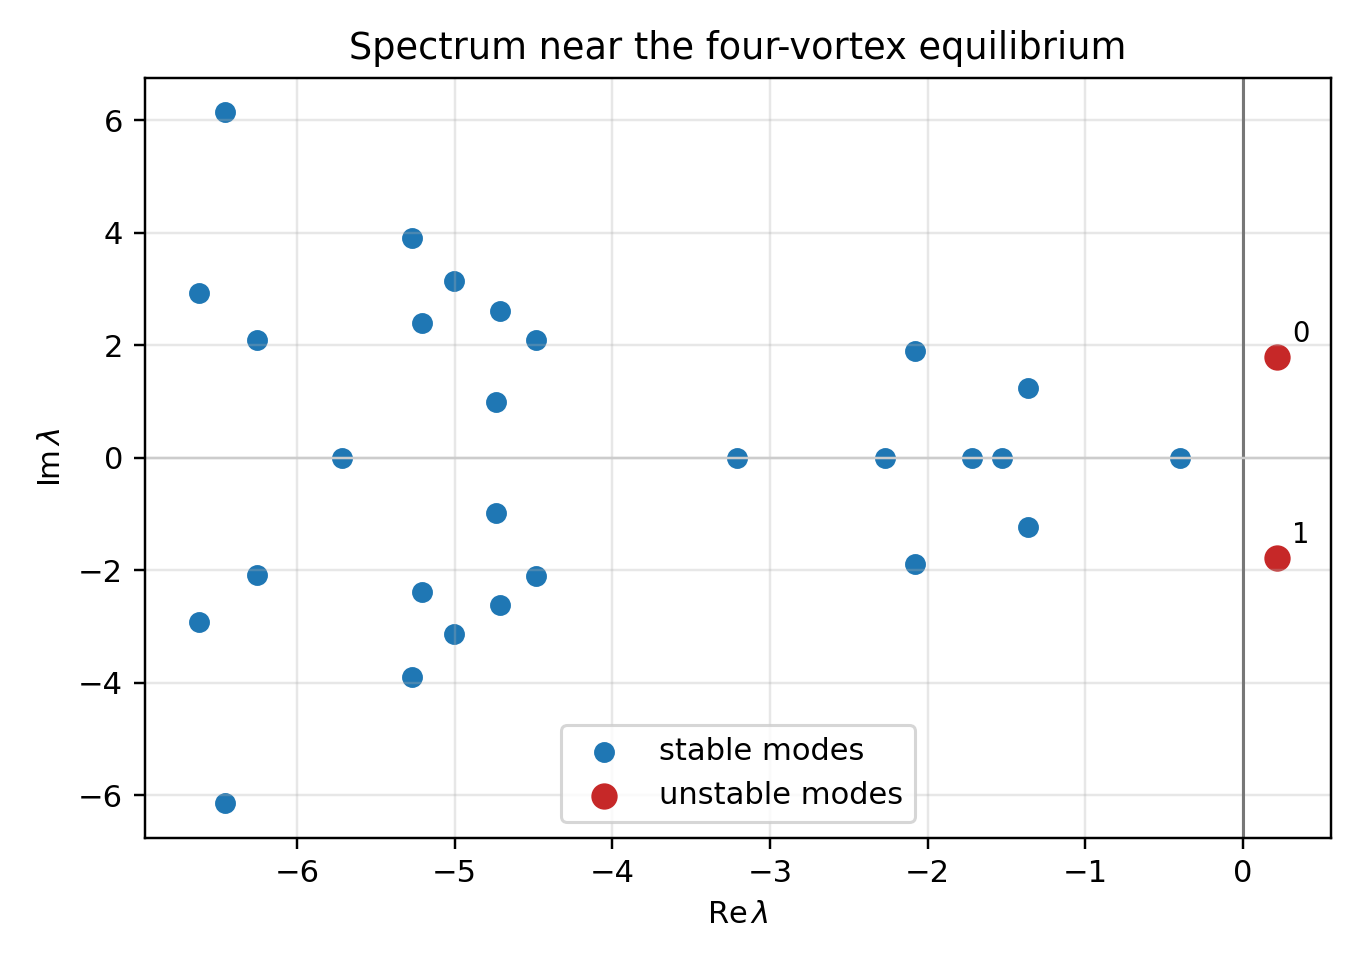
\includegraphics[width=\textwidth]{stability_spectrum.png}\\
            \small спектр \(\mathcal A\)
        \end{column}
        \begin{column}{0.52\textwidth}
            \[
                \lambda_{0,1}
                =
                0.217011
                \pm
                1.786819\,i.
            \]
            \[
                \operatorname{Re}\lambda>0
                \quad\Rightarrow\quad
                \text{линейная неустойчивость.}
            \]
            \[
                \frac{|\operatorname{Im}\lambda|}{2\pi}
                \approx 0.28438.
            \]
            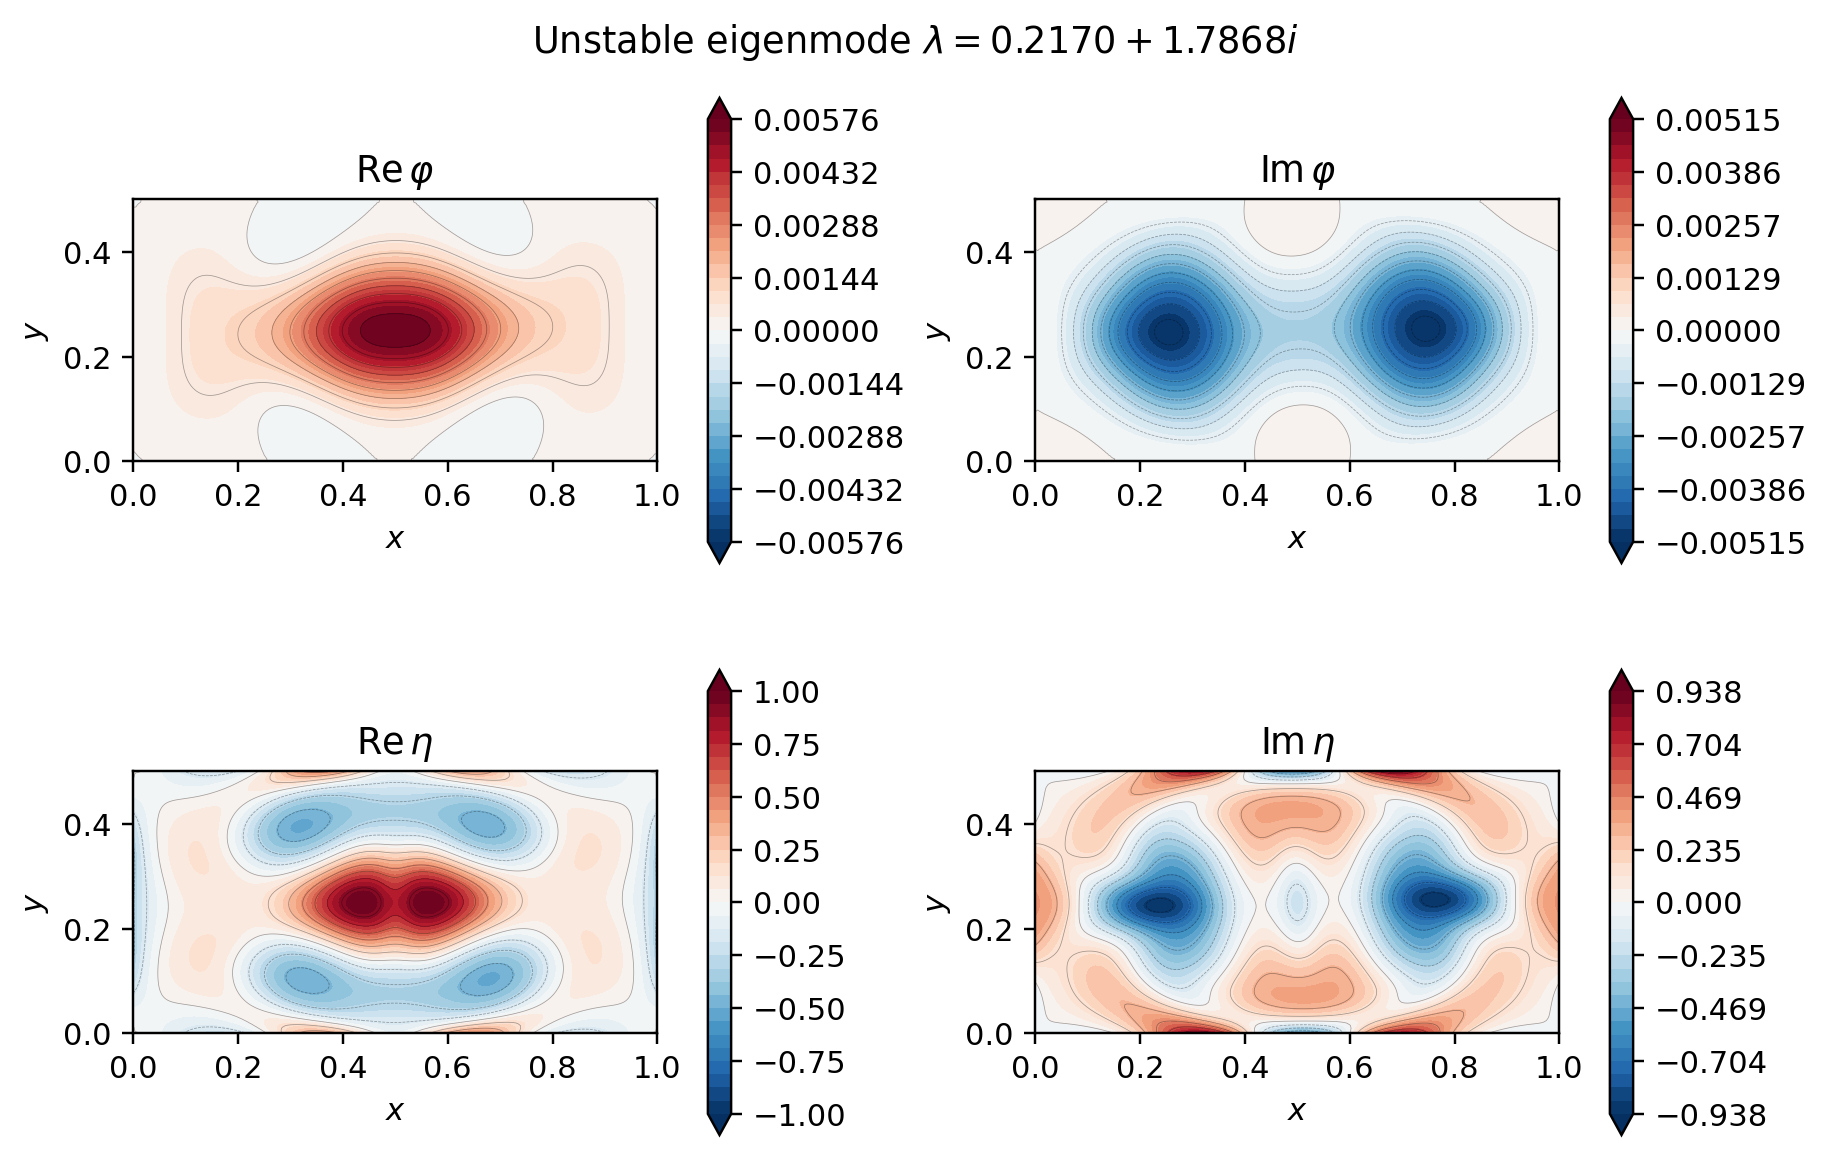
\includegraphics[width=0.95\textwidth]{unstable_mode_000.png}
        \end{column}
    \end{columns}
\end{frame}

\begin{frame}{Вычитание неустойчивой компоненты}
    Комплексная мода \(v=a+ib\) задаёт вещественное подпространство
    \[
        E_{\mathrm{unst}}
        =
        \operatorname{span}\{\operatorname{Re}v,\operatorname{Im}v\}.
    \]
    Для отклонения от стационара
    \[
        r(t)=U(t)-U_*
    \]
    вычисляется проекция:
    \[
        r_{\mathrm{unst}}
        =
        \sum_{\ell=1}^{m}
        \inner{r}{e_\ell}e_\ell.
    \]
    Скорректированное состояние:
    \[
        U_{\mathrm{corr}}=U-r_{\mathrm{unst}}.
    \]
\end{frame}

\begin{frame}{Результат стабилизационного эксперимента}
    \begin{columns}
        \begin{column}{0.48\textwidth}
            \centering
            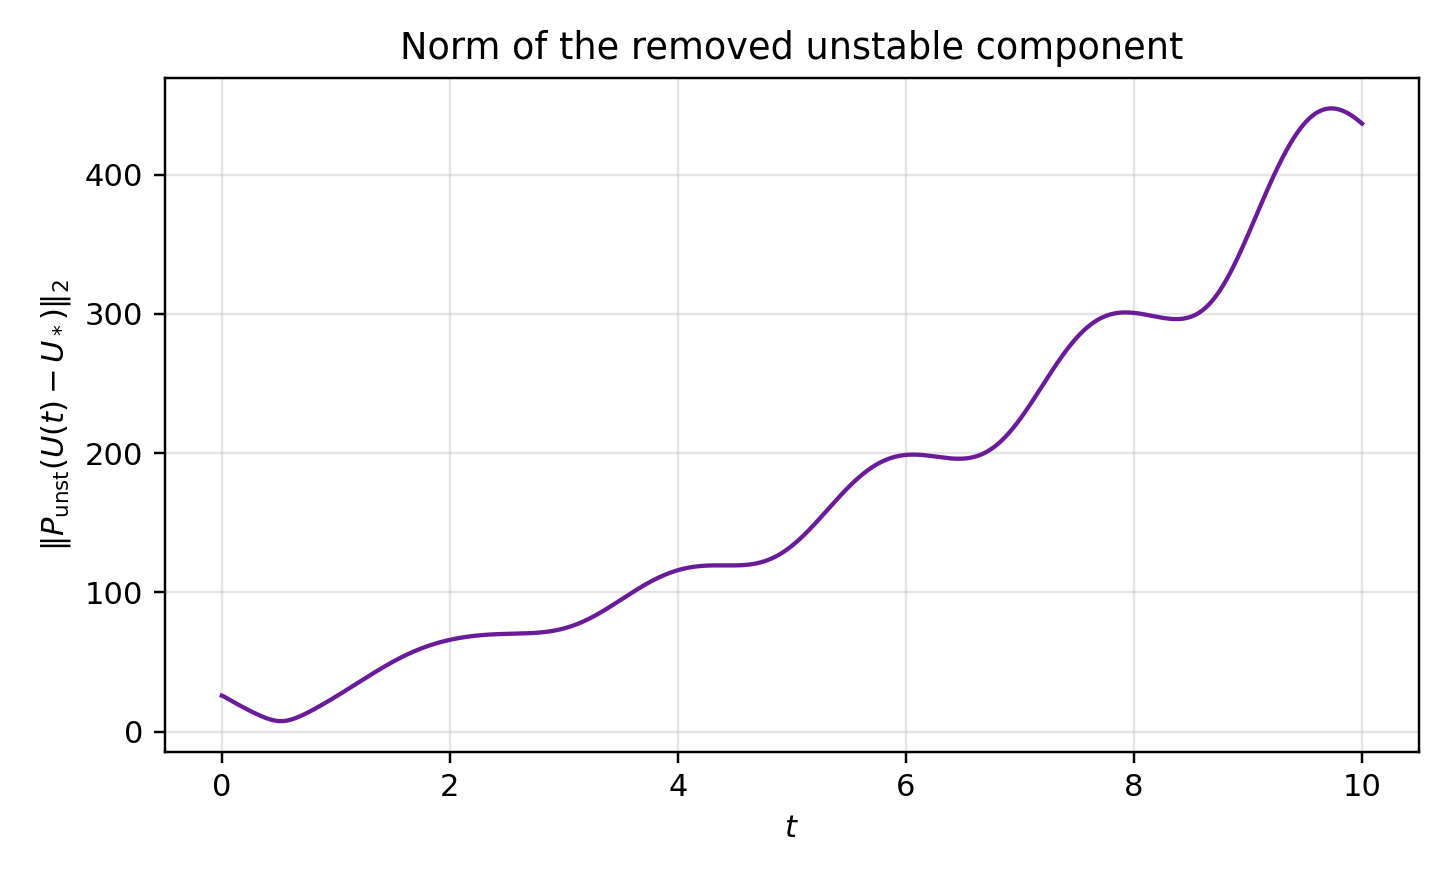
\includegraphics[width=0.92\textwidth]{projection_norm.png}\\
            \small норма проекции на неустойчивое подпространство
        \end{column}
        \begin{column}{0.48\textwidth}
            \centering
            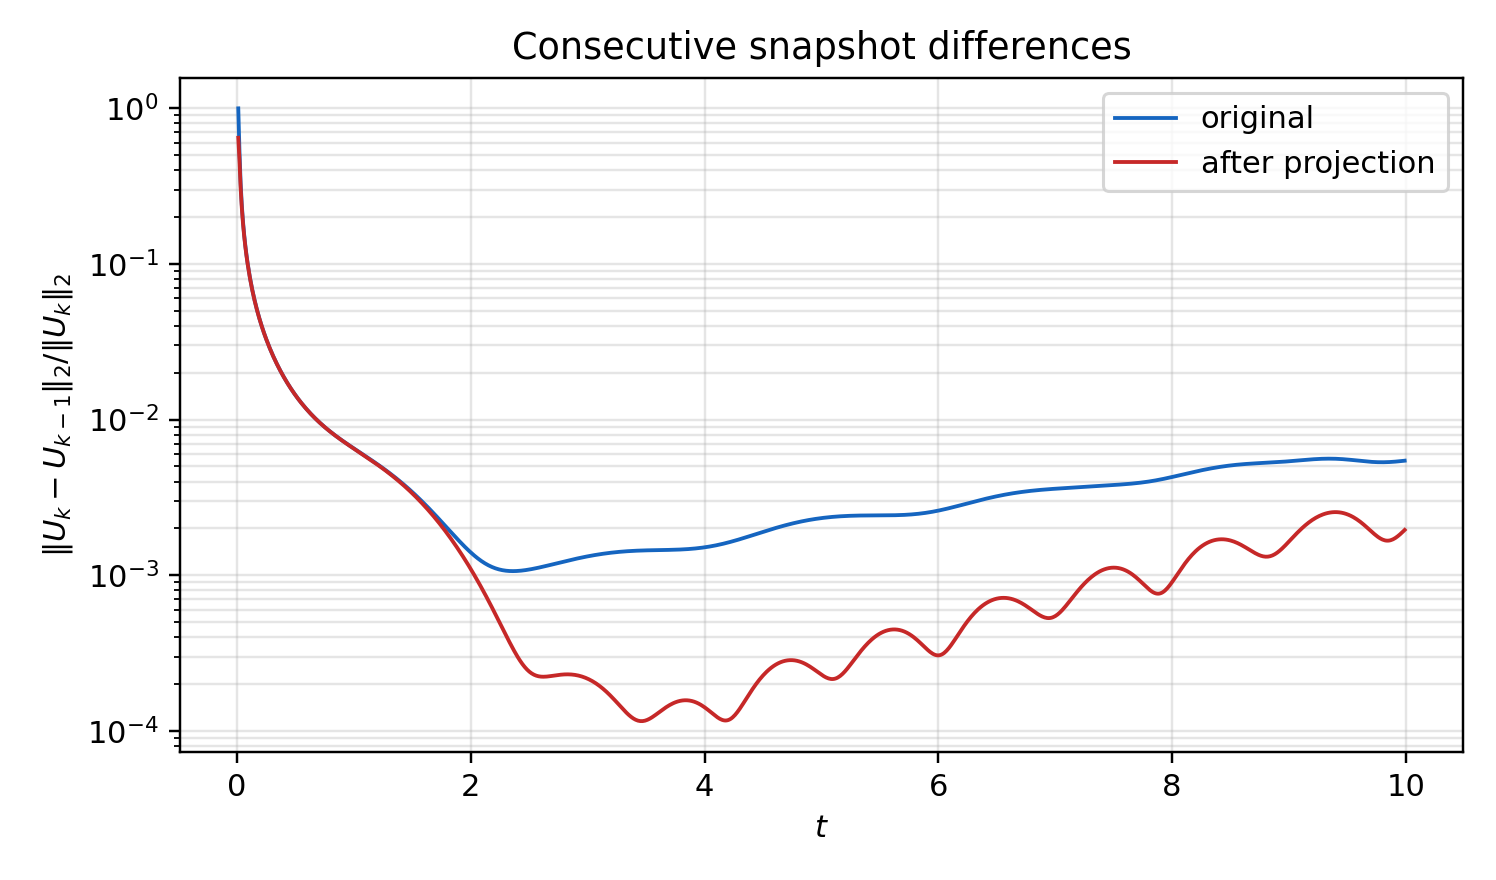
\includegraphics[width=0.92\textwidth]{raw_filtered_difference.png}\\
            \small сравнение исходной и скорректированной динамики
        \end{column}
    \end{columns}
\end{frame}

\begin{frame}{Отклонение от четырёхвихревого состояния}
    \centering
    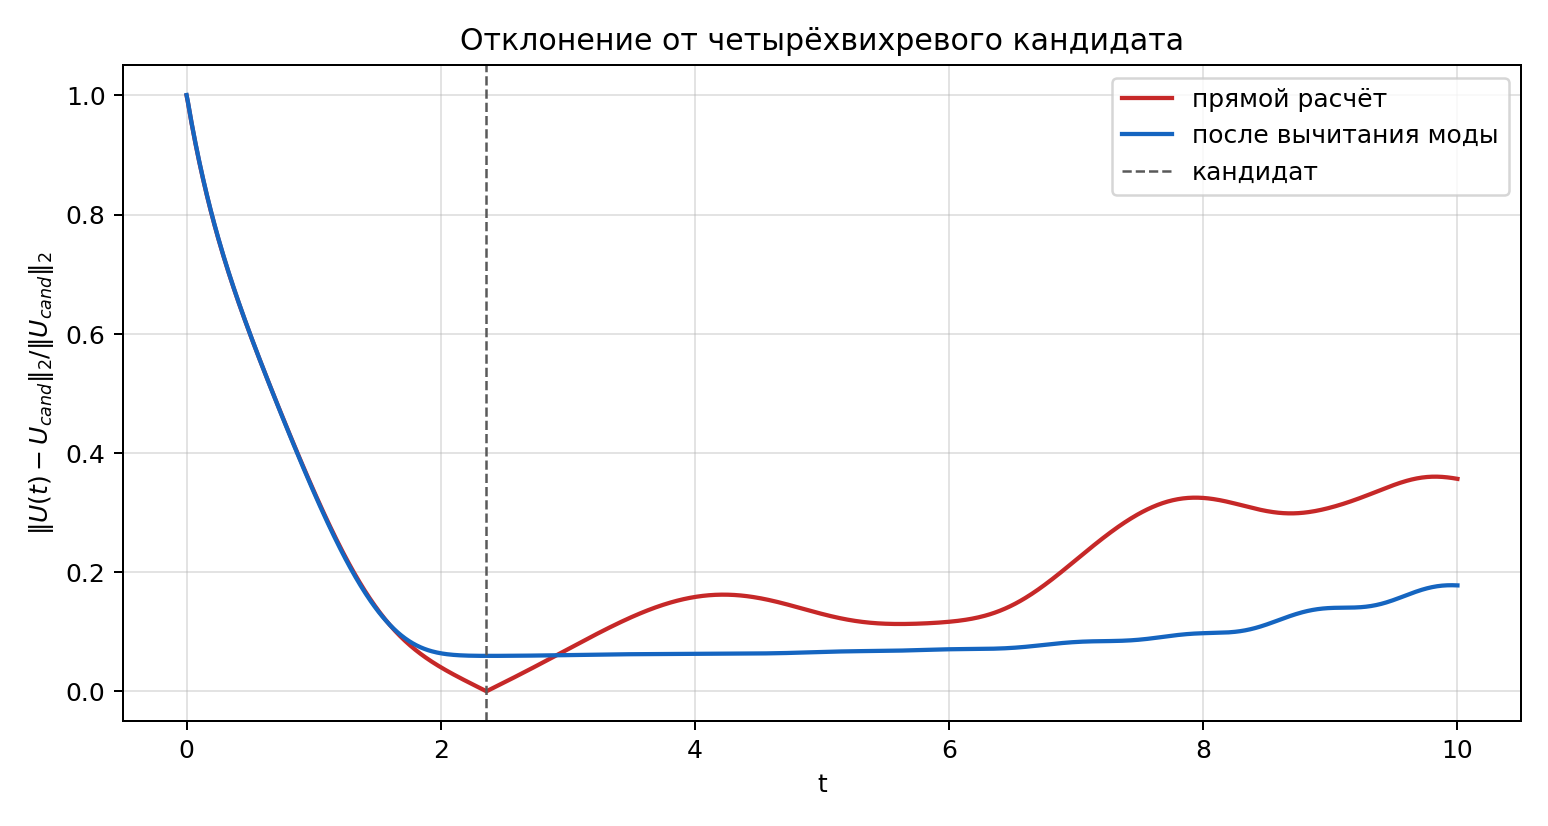
\includegraphics[width=0.70\textwidth]{state_deviation_raw_filtered.png}\\
    \vspace{0.3em}
    \small
    Кандидат:
    \[
        U_{\mathrm{cand}}=U(t_{\mathrm{cand}}),
        \qquad
        t_{\mathrm{cand}}=2.36001,\quad n_{\mathrm{cand}}=236000.
    \]
    Он выбран как сохранённый снимок с минимальной разностью между соседними сохранёнными состояниями.
    На графике:
    \[
        d(t)=
        \frac{\norm{U(t)-U_{\mathrm{cand}}}_2}
             {\norm{U_{\mathrm{cand}}}_2},
        \qquad U=(\psi,\omega).
    \]
\end{frame}

\begin{frame}{Динамика до и после коррекции}
    \begin{columns}
        \begin{column}{0.48\textwidth}
            \centering
            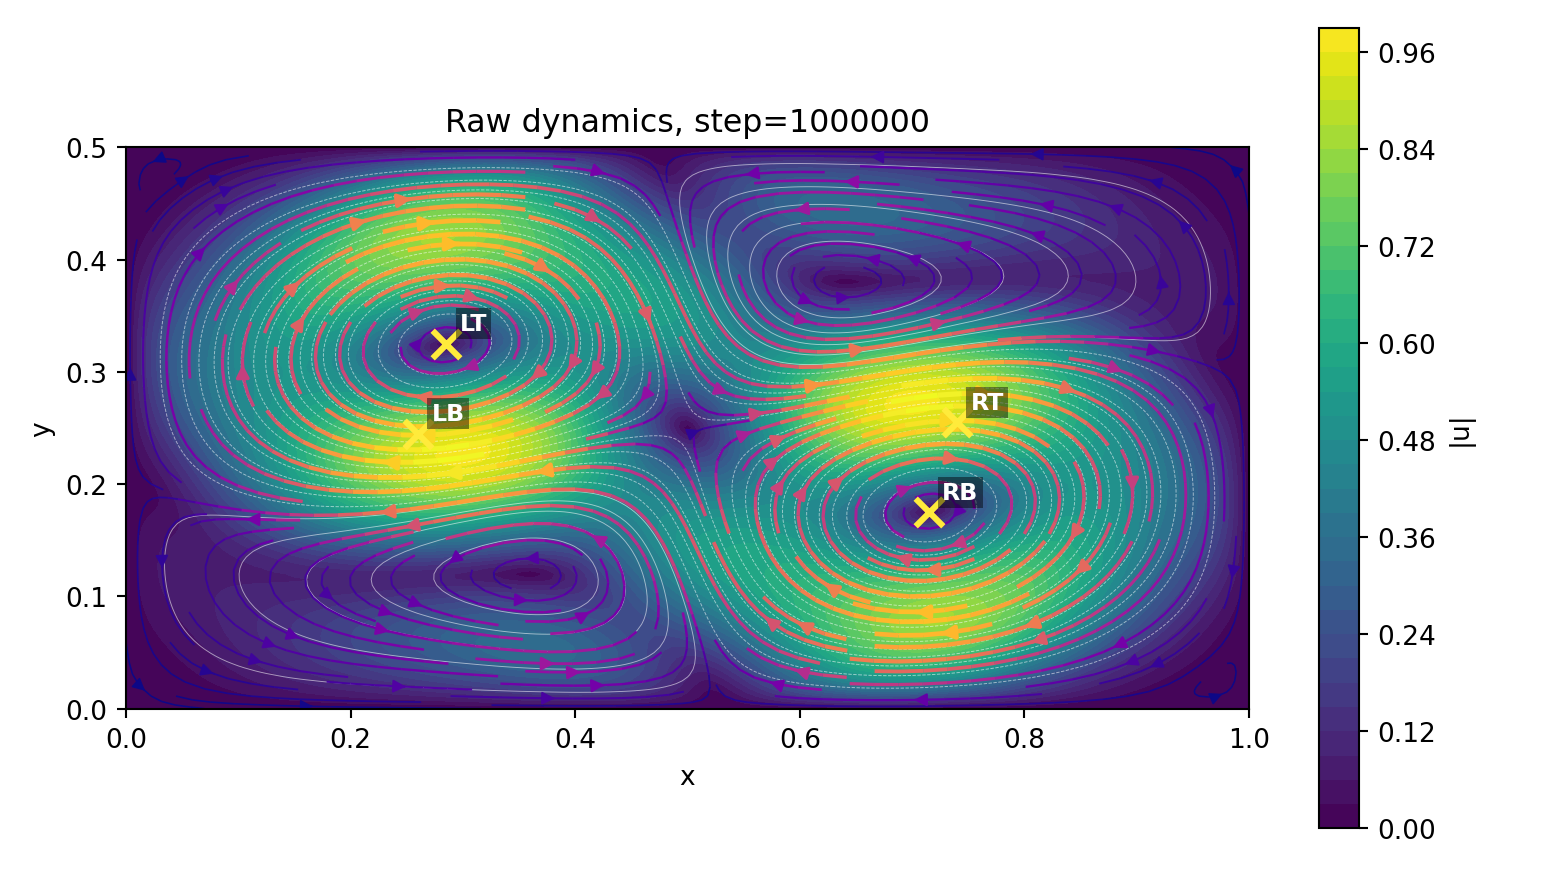
\includegraphics[width=0.92\textwidth]{pulsation_raw_1000000_centers.png}\\
            \small исходная динамика, шаг \(10^6\)
        \end{column}
        \begin{column}{0.48\textwidth}
            \centering
            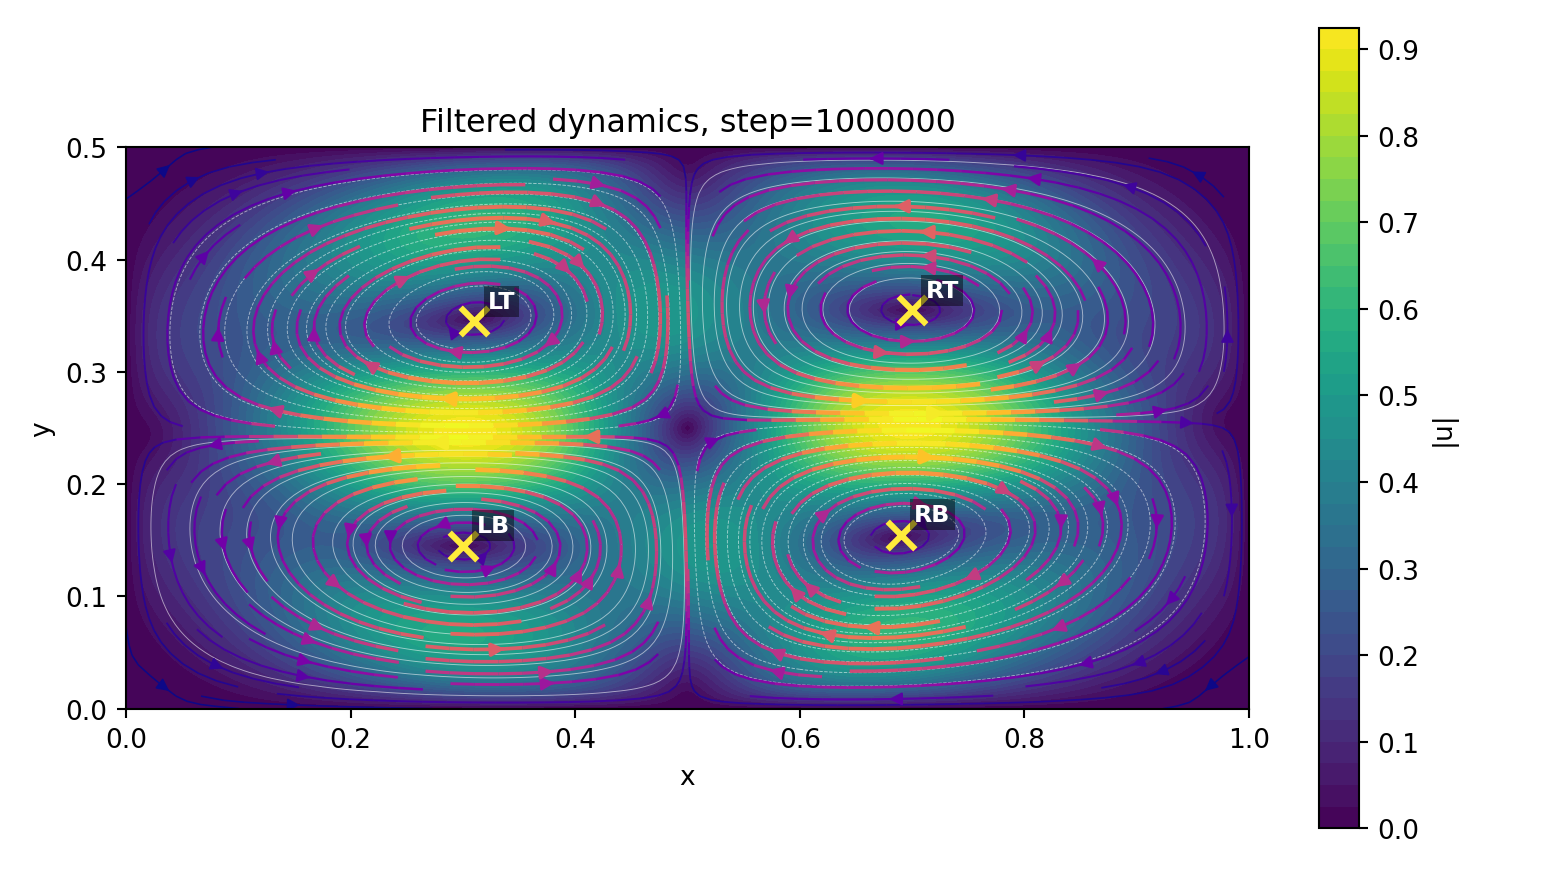
\includegraphics[width=0.92\textwidth]{pulsation_filtered_1000000_centers.png}\\
            \small после вычитания неустойчивой компоненты
        \end{column}
    \end{columns}
\end{frame}

\begin{frame}{Координаты центров четырёх вихрей}
    \centering
    \scriptsize
    \resizebox{0.98\textwidth}{!}{%
    \begin{tabular}{@{}ccccc@{}}
        \toprule
        Ячейка &
        ориентир \(2\times2\) &
        кандидат \(t=2.36001\) &
        прямой расчёт \(t=10\) &
        после коррекции \(t=10\) \\
        \midrule
        LB & \((0.250,\ 0.125)\) & \((0.325,\ 0.140)\) & \((0.260,\ 0.245)\) & \((0.300,\ 0.145)\) \\
        RB & \((0.750,\ 0.125)\) & \((0.690,\ 0.155)\) & \((0.715,\ 0.175)\) & \((0.690,\ 0.155)\) \\
        LT & \((0.250,\ 0.375)\) & \((0.310,\ 0.345)\) & \((0.285,\ 0.325)\) & \((0.310,\ 0.345)\) \\
        RT & \((0.750,\ 0.375)\) & \((0.675,\ 0.360)\) & \((0.740,\ 0.255)\) & \((0.700,\ 0.355)\) \\
        \bottomrule
    \end{tabular}
    }
    \vspace{0.7em}

    \small
    В прямом расчёте центры диагональных ячеек смещаются к центральной линии.
    После вычитания неустойчивой компоненты координаты возвращаются ближе к четырёхвихревому кандидату.
\end{frame}

\begin{frame}{Итоги}
    \begin{itemize}
        \item Построена численная схема в переменных \((\psi,\omega)\) с факторизацией по направлениям и прогонками.
        \item Для задачи о каверне на сетке \(601\times601\) получено совпадение координат центров вихрей с литературными данными.
        \item В четырёхвихревой задаче найдено стационарное состояние и проведён спектральный анализ линеаризованного оператора.
        \item Найдена неустойчивая комплексно-сопряжённая пара
        \[
            \lambda=0.217011\pm1.786819i.
        \]
        \item Вычитание проекции на неустойчивое подпространство уменьшает уход решения от четырёхвихревой структуры.
    \end{itemize}
\end{frame}

\end{document}
